%Seccion "Resumen"
%
\chapter{Combined index notation for finite element analysis}

\section{Combined index notation for finite element analysis}
In the formulation of finite element methods it is customary to start from expressions written in index notations like:


\[ \delta W = \intL_V \sigma_{ij} \delta u_{i,j} \dd{V} \]


and then proceed to introduce discretization or approximations via interpolation theory. In this case it is useful to combine index notation to describe the physical tensorial fields and at the same time the superposition implicit in interpolation schemes. In this appendix we clarify the use of such combined index notation.

\subsection{Index notation of Cartesian tensor fields}

In index notation vector and tensor fields are represented by a letter defining 
the name of the field and a set of different subscripts (or index). The 
number of different indices associated to the letter indicates whether the 
field is a vector (1 index), a second order tensor (2 indices), a third order 
tensor (3 indices) as in:
\[u_i , \sigma_{ij} , C_{ijk}\]

and further clarified next.
 
Consider a vector $\overset\rightharpoonup u$ represented in a Cartesian reference system in terms of its scalar components $u_x , u_y , u_z$. The following representations of the vector are equivalent:

\[u_i\leftrightarrow\begin{bmatrix}u_x&u_y&u_z\end{bmatrix}\leftrightarrow\overset\rightharpoonup u=u_x\widehat i+u_y\widehat j+u_z\widehat k.\]

In the first case, the vector is denoted by the letter $u$ and by the subscript $i$ which represents in condensed form the scalar components $\begin{bmatrix}u_x&u_y&u_z\end{bmatrix}$ of the vector.

Similarly, consider a second order tensor $\overset{\rightharpoonup(2)}\sigma$ represented in a cartesian reference system in terms of its scalar components $\sigma_{xx} , \sigma_{xy}, \sigma_{xz} , \sigma_{yx}, \sigma_{yy}, \sigma_{yz}, \sigma_{zx}, \sigma_{zy}, \sigma_{zz}$. The following representations of the tensor are equivalent:

\[\sigma_{ij}\leftrightarrow\begin{bmatrix}\sigma_{xx}&\sigma_{xx}&\sigma_{xx}\\\sigma_{xx}&\sigma_{xx}&\sigma_{xx}\\\sigma_{xx}&\sigma_{xx}&\sigma_{xx}\end{bmatrix}\leftrightarrow\overset{\rightharpoonup(2)}\sigma.\]

Note that each free or different subscript associated to a letter is a condensed representation of normal scalar components along a basis $\widehat i-\widehat j-\widehat k$. Accordingly, in the case of the second order tensor the subscript $i$ represents variation through $x-y-z$ and subscript $j$ represents variation through $x-y-z.$

\subsection{The summation convention}
In the context of indicial notation subscripts which appear repeated (forming pairs) are used to represent summation. The most simple example is the representation of the dot product between two vectors which can be represented in the following alternative forms:

\[\overrightarrow u\cdot\overrightarrow w\leftrightarrow u_xw_x+u_yw_y+u_zw_z\leftrightarrow\sum_{i=1}^3u_iw_i\leftrightarrow u_iw_i.\]

Accordingly repeated indices represent summation over the range of variation of the index.

\subsection{Indicial notation in interpolation}
From interpolation theory we know that a function $f(x)$ can be approximated in terms of $n$ known values of the solution $\begin{bmatrix}f^1&f^2&...f^n\end{bmatrix}$ using a superposition like

\[f(x)=L^1(x)f^1+L^2(x)f^2+...+L^n(x)f^n\]

and where the terms $L^k s$ are $n$ interpolation functions of order $n-1$. This approximated function can also be represented in terms of indicial notation where we now use capitalized superscripts to refer to the components of the interpolation set as follows:

\[f(x)=L^Q(x)f^Q.\]


In the expression above the approximated function represents a scalar quantity varying over a one-dimensional domain with independent variable $x.$. In the case of approximation via interpolation theory of vector or tensor valued functions we will have subscripts indicating the scalar components of the vector or tensor field and superscripts representing the interpolation polynomials. Using explicit notation a vector function $u_i (x,y,z)$ varying over a three-dimensional space with independent variables $x,y,z$ would be represented like:


\[
\begin{array}{l}u_x(x,y,z)=N^1(x,y,z)u_x^1+N^2(x,y,z)u_x^2+...+N^n(x,y,z)u_x^n\\u_y(x,y,z)=N^1(x,y,z)u_y^1+N^2(x,y,z)u_y^2+...+N^n(x,y,z)u_y^n\\u_z(x,y,z)=N^1(x,y,z)u_z^1+N^2(x,y,z)u_z^2+...+N^n(x,y,z)u_z^n.\end{array}
\]

In this representation it has been assumed that each component $u_x$, $u_y$ and $u_z$ has been approximated using the same interpolation space. In the generalization of the indicial notation to the interpolation of the vector valued function we will associate the subscript, representing the scalar components of the field to the interpolation polynomials. Thus the above expression would be written like:

\[u_i\;(x,y,z)\;=\;N_i^Q(x,y,z)u^Q\]

or 

\[u_i(\overrightarrow x)\;=N_i^Q(\overrightarrow x)u^Q\]

after considering $\overrightarrow x \equiv x,y,z.$


The subscript $i$, representing the physical components of the vector field $u_i$ has been carried out as a subscript to the shape function $N^Q$ for the nodal point $Q$, while the term $u^Q$ refers to the scalar components of the field $u_i$ at the nodal point $Q$. The main advantage in this notation is the possibility of conducting further operations, as required in the derivation of very general finite element algorithms, while combining physical and discrete information.

\paragraph*{Example}

In the expression

\[ \delta W = \intL_V \sigma_{ij} \delta u_{i,j} \dd{V} \]

assume that the primary variable is the displacement field $u_i$ in such a way that at the nodal point $Q$ the displacement vector $u^Q$ is known. Write the interpolated version of $\delta W.$

First, let us write the interpolated approximation to the displacement field $\delta u_i$ carrying the subscript to the shape functions:

\[\delta u_i(\overrightarrow x)\;=N_i^Q(\overrightarrow x)\delta u^Q.\]

To write the interpolated version of $\delta u_{i,j}$ we note that in the expression above the spatial variation of the field has been assumed by the shape function so we just extend the derivative with respect to $x_j$ to these functions to obtain the following interpolated version of the second order tensor field $\delta u_{i,j}$:

\[\delta u_{i,j}(\overrightarrow x)\;=N_{i,j}^Q(\overrightarrow x)\delta u^Q.\]

Making

\[B_{ij}^Q(\overrightarrow x)\equiv N_{i,j}^Q(\overrightarrow x) \]

the above can be written like:

\begin{equation} 
\delta u_{i,j}(\overrightarrow x)\;=B_{ij}^Q(\overrightarrow x)\delta u^Q.
\label{B_strain}
\end{equation}

In \cref{B_strain}, the term $B_{ij}^Q(\overrightarrow x)$ is an interpolation function (which is indicated by the superscript $Q$) associated to a second order tensor (which is indicated by the subscripts $ij$). It must be recognized that $B_{ij}^Q(\overrightarrow x)$ are not independent shape functions but just derivatives of the primary interpolation polynomials $N^Q (x,y)$.

Consider now the stress-strain relationship in theory of elasticity relating the stress tensor $\sigma_{ij}$ to the strain tensor $\epsilon_{ij}$ through the elastic constitutive tensor $C_{ijkl}$as:

\[\sigma_{ij} = C_{ijkl} \epsilon_{kl}.\]

In the above the strain tensor $\epsilon_{ij}$ is given by a combination of space derivatives of the displacement field $u_i$ like

\[ \varepsilon_{ij}=\frac12(u_{i,j}+u_{j,i}) \]

which can be written like


\[ \epsilon_{ij}(\overrightarrow x)\;= \frac12 [B_{ij}^Q(\overrightarrow x) + B_{ji}^Q(\overrightarrow x) ]   u^Q \equiv H(\overrightarrow x)_{ij}^Q u^Q \]

Using the above set of results in $\delta W $ gives:

\begin{equation} 
\delta W=\delta u^Q\int_VH_{ij}^QC_{ijkl}H_{kl}^P\operatorname dVu^P
\label{discrete}
\end{equation}

which is the final discrete version of $\delta W $.

\begin{tcolorbox}
In the indicial representation of a tensor quantity an index which does not repeat itself in the expression is termed a {\bf free index} and the number of non-repeated free indices appearing in the expression gives the expression order. By contrast, repeated indices appearing in the expression are termed {\bf dummy indices} and they imply summation.
\end{tcolorbox}

\paragraph*{Problem: Discretization of the principle of virtual displacements from theory of Elasticity}

The principle of virtual displacements in the linearized theory of elasticity is given by:


\begin{equation} 
\intL_V \sigma_{ij} \delta u_{i,j} \dd{V} - \intL_V f_i \delta u_i \dd{V} - \intL_{S_t} t_i^n \delta u_i \dd{S} = 0.
\label{pvw_2}
\end{equation}

and where $u_i$ is the displacement field; $\epsilon_{ij}$ is the strain field and $\sigma_{ij}$ is the stress field satisfying the following relations

\[ \varepsilon_{ij}=\frac12(u_{i,j}+u_{j,i}) \]

and

\[\sigma_{ij} = C_{ijkl} \epsilon_{kl}\]

where $C_{ijkl}$ is a fourth-order tensor whose terms are material constants. Also $f_i$ and $t_i^n$ are the body forces and the surface traction vectors.

Assuming that in a finite element method the displacement field $u_i$ is approximated via interpolation like:

\[ u_i(\overrightarrow x)\;=N_i^Q(\overrightarrow x)u^Q.\]

\begin{itemize}
\item Write the discrete version of \cref{pvw_2}
\item Write the term $K^{QP} = \int_VH_{ij}^QC_{ijkl}H_{kl}^P\operatorname dV$ in matrix form and implement it in a python script.
\end{itemize}

\newpage

\chapter{Generalized boundary value problems}
%\section{Generalized boundary value problems from a balance law}
In this section we use as problem to be solved via the finite element algorithm the case of general initial boundary value problem (I-BVP). In the first part of this appendix we will introduce the differential formulation given in terms of a set of governing equations and properly specified boundary conditions. The resulting equations are obtained after using a generalized balance law. Following this classical and well known approach we formally re-state these equations in the so-called strong form. Subsequently we re-write and prove an equivalent form of the balance law in the form of an integral representation highly friendly for a numerical solution. Since in the integral description of the problem the order of the derivatives in the field functions decreases by one, the resulting statement is called a weak formulation. 

\section{Governing equations}
Let $\dd{S}$ be a differential surface element, $\dd{V}$ a differential volume element, $u(\vb{x},t)$ a scalar (or vector) function of space and time. The flux or rate of flow of the quantity $u(\vb x, t)$ through $\dd{S}$ at time $t$ is defined like
\[p(\vb x)\grad u \cdot \hat n \dd{S} \enspace ,\]
where $p(\vb x)$ is a positive function, assumed known and time independent. Similarly, the time rate of change of $u(\vb x, t)$ in an element $\dd{V}$ is given by
\[\rho (\vb x)\pdv{u}{t} \dd{V} \enspace ,\]
where once again $\rho (\vb x)$ is a known, given, time independent positive function. Additional effects occurring in the element $\dd{V}$ at the time $t$ can be expressed like
\[H(\vb x, t)\dd{V} \equiv  - q(\vb x)u(\vb x, t) + \hat F(\vb x,t)\]
where $\hat F(\vb x, t) = \rho (\vb x)F(\vb x, t)$. In the above the term $q u$ represents internal effects due to changes proportional to $u$ while $\hat F(\vb x, t)$ are other external influences in the medium.

Balancing the internal and external changes yields
\[\int\limits_V \rho (\vb x)\pdv{u}{t}\dd{V} = \int\limits_S p(\vb x)\vb \grad u \cdot \hat n\dd{S}  + \int\limits_V H(\vb x, t)\dd{V} \enspace ,\]
or equivalently
\[\int\limits_V \rho (\vb x)\pdv{u}{t}\dd{V} = \int\limits_S p(\vb x)\vb \grad u \cdot \hat n\dd{S}   - \int\limits_V q(\vb x)u(\vb x, t)\dd{V}  + \int\limits_V \rho (\vb x)F(\vb x, t)\dd{V} \enspace .\]

Using the divergence theorem as
\[\int\limits_S p(\vb x) \grad u \cdot \hat n \dd{S}  = \int\limits_V \vb \div  (p\vb \grad u)\dd{V}\]
yields after substitution
\[\int\limits_V \left[\rho (\vb x)\pdv{u}{t} - \div (p(\vb x)\grad u) + q(\vb x)u(\vb x, t) - \rho (\vb x)F(\vb x, t)\right]\dd{V}  = 0\]
Assuming a continuous integrand, the arbitrariness of $V$ implies
\[\rho (\vb x)\pdv{u}{t} - \div(p(\vb x)\grad u) + q(\vb x)u(\vb x, t) - \rho (\vb x)F(\vb x, t) = 0\]

Letting
\[\mathcal{L} \equiv  - \div p(\vb x)\grad + q(\vb x)\]
allows us to write the generalized set of partial differential equations like:

\begin{equation}
\rho(\vb x) \pdv{u(\vb x, t)}{t} + \mathcal{L}u(\vb x, t) = \rho (\vb x)F(\vb x, t) \enspace .
\label{eq:GenPDE}
\end{equation}

These are categorized as:
\begin{itemize}
    \item Hyperbolic;
    \[\rho(\vb x) \pdv[2]{u(\vb x, t)}{t} + \mathcal{L}u(\vb x,t) = 0\]

    \item Parabolic;
    \[\rho(\vb x) \pdv{u(\vb x,t)}{t} + \mathcal{L}u(\vb x, t) = 0\]

    \item Elliptic
    \[\mathcal{L}u(\vb x, t) = \rho (\vb x)F(\vb x, t) \enspace .\]
\end{itemize}

It is convenient to show that $\mathcal{L}$ satisfies the \emph{symmetry} condition
\[\int\limits_V \mathcal{L}(u)v\dd{V} =  \int\limits_V \mathcal{L}(v)u \dd{V}\]
and that the operator is positive definite, that is
\[\int\limits_V \mathcal{L}(u)u\dd{V}  > 0, \quad \forall u \enspace .\]

\subsection{Strong form}
The strong form for the generalized boundary value problem formulated above can now be explicitly written as follows.

Given $\rho(\vb x)$, $q(\vb x)$, $p(\vb x)$, $F(\vb x, t)$ and $\bar u (\vb x , t)$ find $u(\vb x , t):V \to \mathbb{R}$ such:
\[\rho(\vb x) \pdv{u}{t} - \div \left[p(\vb x) \grad u\right] + q(\vb x) u(\vb x, t) - \rho(\vb x) F(\vb x, t) = 0 \quad \forall \vb x \in V \]
and
\begin{align*}
    &u = \bar u \quad \forall \vb x \in S_u\\
    &p(\vb x)u_{,i} \hat n_i= B(\vb x,t)\quad \forall \vb x \in  S_t \enspace .
\end{align*}


In the FEM we will look for approximate solutions to $u$ subject to the following conditions:
\[u = \bar u \quad \forall \vb x \in S_u \quad \text{(Essential boundary conditions)}\] 
and
\[\int\limits_S \left(\pdv{u}{x_j}\right)^2 \dd{S} < \infty \enspace ,\]
which corresponds to the functions being square integrable. We will denote this space by $\mathbb{H}$ .

The space of functions satisfying the above two conditions will be denoted by $\zeta$ and termed the space of trial functions, formally defined like:
\[\zeta  = \left\{ u \mid u \in \mathbb{H},u = \bar u \quad \forall\vb x  \in S_u \right\}\]

On the other hand, to validate (or test) the correctness of the approximated or proposed trial functions $u$ it is also necessary to introduce test functions $w$ which are arbitrary except that they satisfy the following conditions:
\[w = 0\quad \forall \vb x \in S_u\] 
and
\[\int\limits_S \left(\pdv{w}{x_j}\right)^2 \dd{S} < \infty \enspace ,\]
which corresponds to the functions being square integrable. The space of functions satisfying the above two conditions will be denoted by $\pounds$ and termed the space of test functions, formally defined like:
\[\pounds  = \left\{w \mid w \in \mathbb{H},w = 0 \quad \forall \vb x \in S_u\right\}\]

\subsection{Weak form}
Given $\rho(\vb x)$, $q(\vb x)$, $p(\vb x)$, $F(\vb x, t)$ and $\bar u (\vb x , t)$ find $u(\vb x , t):V \to \mathbb{R}$ and $\forall w \in \pounds$ such:
\begin{align*}
\int\limits_V p(\vb x) u_{,i}\, w_{,i}\dd{V} - \int\limits_{S_t} B(\vb x, t)w \dd{S}  + \int\limits_V q(\vb x)u(\vb x, t)w\dd{V}  &+ \int\limits_V \rho(\vb x)\pdv{u}{t}w \dd{V} \\& - \int\limits_V \rho(\vb x) F(\vb x, t)w\dd{V} = 0
\end{align*}
and
\[u = \bar u\quad \forall\vb x \in S_u \enspace .\]

\subsection{Equivalence between the strong and weak forms}
\begin{multline}
    -\int\limits_V [p(\vb x)u_{,i}]_{,i}w \dd{V} + \int\limits_{S_t} [p(\vb x)u_{,i}] \hat n_i w\dd{S} - \int\limits_{S_t} B(\vb x, t)w\dd{S}\\
    + \int\limits_V q(\vb x)u(\vb x, t)w \dd{V}  + \int\limits_V \rho(\vec x)\pdv{u}{t}w\dd{V} - \int\limits_V \rho(\vb x)F(\vb x, t)w\dd{V} = 0 
\end{multline}

Grouping together common terms yields
\begin{align*}
&\int\limits_V \left\{\rho(\vb x)\pdv{u}{t} - [p(\vb x)u_{,i}]_{,i} + q(\vb x)u(\vb x, t) - \rho(\vb x)F(\vb x, t)\right\} w\dd{V}\\
&+ \int \limits_{S_t} \left\{[p(\vb x)u_{,i}]\hat n_i - B(\vb x, t) \right\} w\dd{S} = 0
\end{align*}
from which
\[\rho(\vb x)\pdv{u}{t} - [p(\vb x)u_{,i}]_{,i} + q(\vb x)u(\vb x, t) - \rho(\vb x)F(\vb x, t) = 0\]
and
\[p(\vb x)u_{,i}\hat n_i = B(\vb x, t)  \quad\forall \vb x \in S_t \enspace .\]

\section{Weighted residual methods}
This section introduces the concept of residual or difference from zero in a differential equation once its solution is approximated. For that purpose we will take as prototype equation the one obtained as our general model of BVP (see \cref{eq:GenPDE}) and recalled here for completeness
\begin{equation}
\rho(\vb x) \pdv{u(\vb x, t)}{t} + \mathcal{L}u(\vb x, t) = \rho (\vb x)F(\vb x, t) \enspace .
\label{eq:GenPDE2}
\end{equation}

We will assume that the actual solution to the generalized BVP given by \cref{eq:GenPDE2} is approximated by $\tilde u(\vb{x})$ through a superposition like
\begin{equation}
\tilde u (\vb{x}) = {N^I}(\vb{x}){u^I}
\label{basicsuper}
\end{equation}
where ${N^I}(\vb{x})$ are interpolating functions and $I$ denotes a superposition index  varying like $I=1,2,...,K$ with $K$ being the number of points where the solution is known. In what follows we will use $u(\vb{x})$ instead of $\tilde u (\vb{x})$ but will keep in mind that we are actually using the approximation given by \cref{basicsuper}. Similarly, in order to keep the discussion simple for the time being we will drop the time effects reducing the generalized PDE to the simple form:
\begin{equation}
\mathcal{L}u(\vb x) = \rho (\vb x)F(\vb x) \enspace .
\label{eq:GenPDE3}
\end{equation}

Now, since we are using the approximation given by \cref{basicsuper} this equation is not strictly satisifed but instead we will have the following ``unbalanced" condition
\[\mathcal{L}u(\vb{x}) - \rho (\vb{x})F(\vb{x}) \equiv R \ne 0\]
where the term $R$ corresponds to a residual error which is to be distributed throughout the solution domain. The so-called weighted residual methods differ in the form in which they distribute the residual between the different $K$ points conforming the computational domain.

Using \cref{basicsuper} in \cref{eq:GenPDE2} and the linearity in the differential operator yields
\[R = \mathcal{L}({N^P}){u^P} - \rho F\, .\]

We can see that the residual $R$ is a function defined over the domain of interest. The residual would be exactly zero for the solution of the differential equation, but it will not be zero in general. Thus, we want to make the function $R$ as close to zero as possible. To make $R$ as small as possible we need a function (a functional) where we can compare different approximation functions. After getting this functional we can minimize its value. For this minimization we could use the norm of the function, another option is to compute a weighted \emph{average} of the function over the domain. This is what we call a weighted residual
\[\Pi[u, w] = \int\limits_V w R(u) \dd{V}\, ,\]
and we want to minimize it by making
\[\var{\Pi}[u, w] = 0\, ,\]

In what follows we will consider different strategies to distribute or weight the residual $R$ over the computational domain.

\subsection{Galerkin method}
In the Galerkin scheme the interpolation functions are used also as weighting functions leading to:
\[\int\limits_V N^Q R\dd{V} = 0 \]
or explicitly
\begin{equation}
  \int\limits_V N^Q \mathcal{L} (N^P)\dd{V} u^P = \int\limits_V N^Q\rho F\dd{V}\, .
  \label{eq:Galer}
\end{equation}

Imposing \cref{eq:Galer} in the $K$ points conforming the computational domain or equivalently ranging $Q$ from $1$ to $K$ leads to the following system of algebraic equation
\begin{equation}
{K^{QP}}{U^P} = {f^Q}
\label{eq:DGaler}
\end{equation}

where $U^P$ is a vector that stores the point values of the function $u$ along te $K$ points of the computational domain, while $f^Q$ stores the corresponding point excitations.

\subsection{Least squares method}
In this method the integral of the square of the residual is minimized with respect to the $K$ point parameters or nodal values of the function. Accordingly,
\begin{align*}
  &\pdv{u^I}\int\limits_V R^2 \dd{V} = 0\\
  &\int\limits_V R \pdv{R}{u^I} \dd{V} = 0\, ,
\end{align*}

The least squares method is a special case of the weighted residual method for the weight functions
\[w^I = \pdv{R}{u^I}\, .\]

Expanding the residual, and considering the operator $\mathcal{L}$ as linear, we obtain
\begin{align*}
  &\pdv{u^I}\int\limits_V [\mathcal{L}(N^P u^P) - \rho F]^2 \dd{V} = 0\\
  &\int\limits_V [\mathcal{L} N^P u^P - \rho F] \mathcal{L}(N^I) \dd{V} = 0\\
 &\int\limits_V \mathcal{L}(N^I) \mathcal{L}(N^P) \dd{V} u^P - \rho \int\limits_V \mathcal{L}(N^I) F \dd{V} = 0
\end{align*}
which can be written like
\begin{equation}
  K^{IP} U^P = f^I
  \label{eq:Dsquares}
\end{equation}

\subsection{Collocation method}
In the collocation method the coefficients of the approximation are determined by forcing the residual to be exactly zero at $K$ points over the computational domain, i.e.,
\[\mathcal{L}(N^I) u^I - \rho F = 0\, ,\]
or
\[\mathcal{L}[N^I(x^J)] u^I - \rho F(x^J) = 0\, ,\]
where $J$ ranges between $1$ and $K$. This equation can be rewritten as a weighted-residual if we consider the residual to be $\delta(x - x^I)$, the Dirac delta function over the selected points

The resulting system of algebraic equation can be written as
\begin{equation}
K^{IP} U^P = f^I\, .
\label{eq:Colo}
\end{equation}

\subsection{Subdomain method}
The zero value of the residual is imposed upon $K$ subdomains
\[\int\limits_{V^I} \mathcal{L}(N^P)\dd{V^I} u^P  - \rho \int\limits_{V^I}  F\dd{V^I}  = 0 \qquad I=1,\cdots,K\, .\]

For instance, for the $N$-th element it follows that
\[\int\limits_{V^N} \mathcal{L}(N^P)\dd{V^N} u^P  - \rho \int\limits_{V^N} F\dd{V^N}  = 0 \qquad P=1,\cdots,K\, .\]

Applying the equation over the $K$ subdomains leads to the discrete system;
\begin{equation}
K^{IP} U^P = f^I \quad \quad I=1,\cdots,K\, .
\label{eq:Subdomain}
\end{equation}

\subsection{Ritz method}
It operates directly upon the variational statement of the problem. For a given functional
\[\Pi  = \Pi (N^Q u^Q)\]
the variational equation reads
\[\var{\Pi}  \equiv \pdv{\Pi}{u^Q} \var{u^Q} = 0\]
from which
\[\pdv{\Pi}{u^Q} = 0\, .\]

\paragraph*{Example: The generalized parabolic equation}
Let us consider the case of the generalized parabolic equation and its discretization following the Galerkin method
\[\rho(\vb x) \pdv{u(\vb x,t)}{t} + \mathcal{L}u(\vb x, t) = 0\]
which can also be written using index notation
\[\pdv{x_i}\left[p(x)\pdv{u}{x_i} \right] + q(x)u + \rho \pdv{u}{t} = \rho F\, 
,.\]

Assuming that $p(x)=1$ yields
\begin{align*}
  &-\int\limits_V N^P N_{,ii}^Q \dd{V} u^Q + \int\limits_V q N^P N^Q\dd{V} u^Q  + \rho \int\limits_V N^P N^Q \dd{V} v^Q\\
     &- \rho \int\limits_V N^P F \dd{V} = 0\\
  &\int\limits_V N_{,i}^P N_{,i}^Q \dd{V} u^Q - \int\limits_S N^P N_{,i}^Q \hat{n}_i \dd{S} u^Q + \int\limits_V q N^P N^Q \dd{V} u^Q\\
    &+ \rho \int\limits_V N^P N^Q \dd{V} v^Q  - \rho \int\limits_V N^P F \dd{V} = 0 \\
  &\int\limits_V \left(N_{,i}^P N_{,i}^Q + q N^PN^Q \right)\dd{V} u^Q  + \rho \int\limits_V N^P N^Q \dd{V} V^Q  =\\
      &\int\limits_S N^P N_{,i}^Q \hat{n}_i \dd{S} u^Q + \rho \int\limits_V N^P F \dd{V}
\end{align*}
which can be written in discrete form as
\[K^{PQ} U^Q + C^{PQ} V^Q = f^p\, .\]

\paragraph*{Example: The wave equation.}
In this case the differential equation reads
\[\div \left[ \frac{1}{\rho} \grad p(\vb{x})\right] - \pdv{t} \left(\frac{1}{\lambda} \pdv{\rho}{t}\right) - q(\vb{x}) = 0\]
where we recognize that
\[\mathcal{L} \equiv \div \left(\frac{1}{\rho} \grad \right) - \pdv{t}\left(\frac{1}{\lambda}\pdv{t}\right)\, .\]

Let
\[p(x) = N^K p^K\]
then
\[\mathcal{L}(p) \equiv \vec \nabla  \cdot \left( {\frac{1}{\rho }\vec \nabla {N^K}{p^K}} \right) - \frac{\partial }{{\partial t}}\left( {\frac{1}{\lambda }\frac{{\partial {N^K}{p^K}}}{{\partial t}}} \right)\]
or in index notation
\[\mathcal{L}(p) \equiv {\left( {\frac{1}{\rho }N_{,i}^K} \right)_{,i}}{p^K} - \frac{\partial }{{\partial t}}\left( {\frac{1}{\lambda }\frac{{\partial {N^K}}}{{\partial t}}} \right){p^K}\]
which is equivalent to
\[\mathcal{L}(p) \equiv \mathcal{L}({N^K}){p^K}\]
using the trial functions as weighting function and recalling the definition of the residual which in this case reads
\[R = \mathcal{L}({N^K}){p^K} - q\, ,\]
and yields
\[\int\limits_V {{N^J}RdV = 0} \quad \quad J=1,2,...,K \]

\[\int\limits_V {{N^J}L({N^K})dV{p^K}}  - \int\limits_V {{N^J}qdV}  = 0\]

\[\int\limits_V {{N^J}{{\left( {\frac{1}{\rho }N_{,i}^K} \right)}_{,i}}dV{p^K} - \int\limits_V {{N^J}\frac{\partial }{{\partial t}}\left( {\frac{1}{\lambda }\frac{{\partial {N^K}}}{{\partial t}}} \right)dV{p^K}} }  - \int\limits_V {{N^J}qdV}  = 0\]

Integrating by parts the first term on the right-hand-side gives us
\[ - \int\limits_V {N_{,i}^J\frac{1}{\rho }N_{,i}^KdV} {p^K} + \int\limits_S {{N^J}\frac{1}{\rho }N_{,i}^K{{\hat n}_i}dS{p^K}}  = \int\limits_V {{N^J}\frac{\partial }{{\partial t}}\left( {\frac{1}{\lambda }\frac{{\partial {N^K}}}{{\partial t}}} \right)dV{p^K}}  + \int\limits_V {{N^J}qdV} \]

\[\int\limits_V {N_{,i}^J\frac{1}{\rho }N_{,i}^KdV} {p^K} + \int\limits_V {{N^J}\frac{1}{\lambda }{N^K}dV{{\ddot p}^K}}  = \int\limits_S {{N^J}\frac{1}{\rho }N_{,i}^K{{\hat n}_i}dS{p^K}}  + \int\limits_V {{N^J}qdV} \]

\[{K^{JK}}{P^K} + {M^{JK}}{{\ddot P}^K} + {f^J} = 0\]

\newpage
\paragraph*{Example: The Navier equations.}
The stress equilibrium equations when written in terms of displacements after using the constitutive tensor and the proper kinematic description take the form:

\[(\lambda  + \mu ){u_{j,ij}} + \mu {u_{i,jj}} + {f_i} = 0 \enspace \]

which are known as the Navier equations and where the differential operator reads

\[L_{ij} \equiv (\lambda  + \mu )\pdv[2]{}{x_i}{x_j} + \mu \pdv[2]{}{x_k}{x_k}\delta_{ij}.\]

Applying this operator to an interpolated version of the displacement field $u_i = N_i^Q u^Q$ gives:

\[L_{ij}(u_j)\equiv R_i(u_j)\]

thus

\begin{align*}
&\mathcal{L}_{ij}(u_j) \equiv (\lambda  + \mu )(N_j^Q u^Q)_{,ij} + \mu (N_j^Q u^Q)_{,kk}\delta_{ij}\\
&\mathcal{L}_{ij}(u_j) \equiv (\lambda  + \mu )N_{j,ij}^Q u^Q + \mu N_{i,kk}^Q u^Q\\
&\mathcal{L}_{ij}(u_j) \equiv \mathcal{L}_{ij}(N_j^Q) u^Q \enspace .
\end{align*}

In the Galerkin scheme we use the trial function as weighting function.
\[R_i \equiv L_{ij}(N_j^Q) u^Q + f_i\]
and we state
\[\int\limits_V N_i^P R_i \dd{V} = 0 \qquad P=1,2,\cdots N\, .\]

Thus
\begin{align*}
&\int\limits_V N_i^P \mathcal{L}_{ij} (N_j^K)\dd{V} u^K  + \int\limits_V N_i^P f_i \dd{V} = 0 \\
&(\lambda  + \mu )\int\limits_V N_i^PN_{j,ij}^K \dd{V} u^K  + \mu \int\limits_V N_i^PN_{i,kk}^K \dd{V} u^K  + \int\limits_V N_i^P f_i \dd{V} = 0
\end{align*}
integrating by parts
\begin{align*}
- (\lambda  + \mu )\int\limits_V N_{i,j}^P N_{j,i}^K \dd{V} u^K + (\lambda  + \mu )\int\limits_S N_i^P N_{j,i}^K \hat{n}_j \dd{S} u^K - \mu \int\limits_V N_{i,k}^P N_{i,k}^K \dd{V} u^K \\
+ \mu \int\limits_S N_i^P N_{i,k}^K \hat{n}_k \dd{S} u^K  + \int\limits_V N_i^P f_i \dd{V} = 0
\end{align*}
which can be written like
\[K^{PQ} U^Q = F^P\]
where
\[K^{PQ} = (\lambda  + \mu )\int\limits_V N_{i,j}^P N_{j,i}^Q \dd{V}  + \mu \int\limits_V N_{i,k}^P N_{i,k}^Q\dd{V} \]
and
\[F^P = \int\limits_S N_i^P t_i^{(\hat n)} \dd{S} + \int\limits_V N_i^P f_i 
\dd{V} = 0 \, .\]



%\newpage
%\section*{Quadratures}
%\section{Gaussian quadratures}
%In the numerical quadrature corresponding to the extended trapezoidal rule written in the form
%
%\begin{equation}
%\int\limits_a^b {f(x)dx \approx \sum\limits_{I = 1}^{npts} {{w^I}f({x^I})} }
%\label{quadra2}
%\end{equation}
%
%the integration points are equidistantly spaced. In a Gaussian quadrature in addition to adjusting the $N$ weighting factors $w^I$ one also leaves as adjustable parameters the location of the $N$ integration points. As a result, there are now $2N$ parameters to adjust in the derivation of an algorithm to numerically approximate the integral of $f(x)$ between $x=a$ and $x=b$ with the maximum accuracy and the minimum number of operations. This class of quadratures provide better precision than those based on Newton-Cotes techniques (such as the trapezoidal rule) when the function to integrate can be appropriately represented by a polynomial. Using a Gaussian quadrature one can integrate functions which are expressible in the form:
%
%\[\int\limits_a^b {w(x)f(x)dx}  \approx \sum\limits_{I = 1}^{npts} {{w^I}f({x^I})}. \]
%
%This particular factorization ${w(x)f(x)}$ is useful since it allows us to write a function as the product of a polynomial $f(x)$ times a known function $w(x)$. This last function can be selected to remove integrable singularities out of the integral. To clarify, consider the following (Gauss-Chebyshev) integral:  
%
%
%\[I = \int\limits_{ - 1}^1 {\frac{{{e^{ - C_x^2}}}}{{\sqrt {1 - {x^2}} }}} dx \equiv \int\limits_{ - 1}^1 {\frac{1}{{\sqrt {1 - {x^2}} }}} {e^{ - C_x^2}}dx\]
%where
%\[w(x) = \frac{1}{{\sqrt {1 - {x^2}} }}\]
%
%and 
%
%\[f(x) = {e^{ - C_x^2}}.\]
%
%Now, making:
%\[g(x) = w(x)f(x)\]
%and
%\[{v^I} = \frac{{{w^I}}}{{w({x^I})}}\]
%
%yields:
%
%\begin{equation}
%\int\limits_{ - 1}^{ + 1} {g(x)dx}  \approx \sum\limits_{I = 1}^{npts} {{v^I}g({x^I})}
%\label{gauss}
%\end{equation}
%
%In general, different Gaussian quadratures are found in the literature reported in terms of tables providing the locations of integration (or Gauss) points and the corresponding weighting factors $w^I$. As an example \cref{ejemplo2} gives abscissas and weighting factors for a 4-point Gaussian quadrature.
%
%\begin{center}
%\begin{tabular}{cc}
%  \hline
%  $x^I$ & $w^I$ \\
%  \hline 
%  $-0.86113$  & $0.34785$  \\
%  $-0.33998$  & $0.65214$  \\
%  $ +0.33998$  & $0.65214$  \\
%  $ +0.86113$  & $0.34785$  \\
%  \hline
%\end{tabular}
%\captionof{table}{Abscissas and weighting factors to compute $\int\limits_{ - 1}^{ + 1} {f(x)dx}$}
%\label{ejemplo2}
%\end{center}
%
%To facilitate coding of these quadratures and allow for approximation of general integrals, it is common to consider a primitive range of integration $[-1.0,+1.0]$ which requires transforming the original integral (including the function and its integration limits)to this primitive integral as discussed in \cref{isopar}. \Cref{fig:quagauss} schematizes the primitive integration range and the corresponding Gauss points denoted by the black $x$s. Transformation of a given integral to the primitive space is discussed at a later section.
%
%\begin{figure}[H]
%\centering
%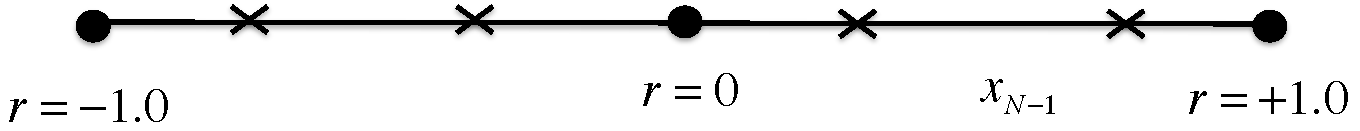
\includegraphics[width=10cm]{img/quagauss.pdf}
%\caption{Schematic reperesentation of a Gaussian quadrature in the primitive range $[-1.0,1.0]$.}
%\label{fig:quagauss}
%\end{figure}
%
%\paragraph*{Example:Derivation of a Gaussian quadrature}
%Let $n=2$ and the integration interval $[a,b]=[-1,+1]$. Find $w^1$, $w^2$ and $x^1$, $x^2$ such the quadrature
%
%
%\[I = \int\limits_{ - 1}^{ + 1} {f(x)dx}  \approx {w^1}f({x^1}) + {w^2}f({x^2})\]
%
%integrated exactly the function  $f(x)$ corresponding to a third order polynomial like:
%
%
%
%\[f(x) = {a_0} + {a_1}x + {a_2}{x^2} + {a_3}{x^3}.\]
%
%Using $f(x)$ in $I$ and stating the integral for each term we have:
%
%
%\[I = \int\limits_{ - 1}^{ + 1} {{a_0}dx}  + \int\limits_{ - 1}^{ + 1} {{a_1}xdx}  + \int\limits_{ - 1}^{ + 1} {{a_2}{x^2}dx}  + \int\limits_{ - 1}^{ + 1} {{a_3}{x^3}dx} \]
%
%where:
%
%\[\int\limits_{ - 1}^{ + 1} {dx}  = 2 = {w^1} \cdot 1 + {w^2} \cdot 1\]
%
%\[\int\limits_{ - 1}^{ + 1} {xdx}  = 0 = {w^1} \cdot {x^1} + {w^2} \cdot {x^2}\]
%
%\[\int\limits_{ - 1}^{ + 1} {{x^2}dx}  = \frac{2}{3} = {w^1} \cdot {({x^1})^2} + {w^2} \cdot {({x^2})^2}\]
%
%\[\int\limits_{ - 1}^{ + 1} {{x^3}dx}  = 0 = {w^1} \cdot {({x^1})^3} + {w^2} \cdot {({x^2})^3}.\]
%
%The resulting system of equations is solved in order to determine the 4 quadrature parameters, namely $w^1$, $w^2$ and $x^1$, $x^2$ giving $w^1 = 1$, $w^2 = 1$, $x^1 =  - \sqrt 3 /3$ and $x^1 =  + \sqrt 3 /3$ which allows us to write the quadrature in the general form:
%
%\[I = \int\limits_{ - 1}^{ + 1} {f(x)dx}  \approx 1.0 \cdot f( - \sqrt 3 /3) + 1.0 \cdot f( + \sqrt 3 /3)\]
%
%which is exact for polynomial functions of order at most 3.
%
%The idea behind Gaussian quadratures can be extended to the integration of higher order polynomials, however its derivation requires an effective method to determine the weighting factors and the abscissas of the Gauss points. The next section discusses a method which is applicable to $2n$-order polynomials, in which advantage is taken from the property of orthogonality existing in certain special polynomials.
%
%\paragraph*{Orthogonal polynomials}
%Two polynomials $P(x)$ and $Q(x)$, where $P(x) \ne Q(x)$ are said to be orthogonal if:
%
%\[\int\limits_a^b {P(x)Q(x)} dx = 0.\]
%
%Particularly, the Legendre polynomials, defined by:
%
%\[P_n(x) = \frac{1}{2^n n!}\frac{d^n}{dx^n}[(x^2 - 1)^n]\]
%
%which at the same time are solution to the equation:
%
%
%\[(1 - {x^2}){y^{''}} - 2x{y^{'}} + n(n + 1)y = 0\]
%
%in the range $[-1,+1]$ satisfy the following orthogonality condition:
%
%\[\int\limits_{ - 1}^{ + 1} {{Q_i}(x)} {P_j}(x)dx = 0\]
%
%where ${{Q_i}(x)}$ is any polynomial function of order $i<j$. 
%
%Besides the orthogonality property, Legendre polynomials have roots in the range $(-1.0,+1.0)$ which are different and symmetrical with respect to zero. This last condition make the roots useful in the derivation of quadratures for the integration of polynomial functions of order less than $2n$. For instance, the second Legendre polynomial given by:
%
%\[{P_2}(x) = {x^2} - \frac{1}{3}\]
%
%has roots ${x^1} =  - \frac{{\sqrt 3 }}{3}$ and ${x^2} =  + \frac{{\sqrt 3 }}{3}$ which correspond to integration points for an exact quadrature of order 3.
%
%\paragraph*{Theorem}
%
%Let $\left\{ {{x^1},{x^2},...,{x^n}} \right\}$ the roots of the Legendre polynomial ${P_n}(x)$ of order $n$; let \[{w^I} = \int\limits_{ - 1}^{ + 1} {\prod\limits_{J = 1}^n {\frac{{x - {x^J}}}{{{x^I} - {x^J}}}} dx} \] and let $f(x)$ be any polynomial function of order less than $2n$, then:
%
%\begin{equation}
%I = \int\limits_{ - 1}^{ + 1} {f(x)dx}  = \sum\limits_{I = 1}^n {{w^I}f({x^I})}.
%\label{Legendre}
%\end{equation}
%
%
%\paragraph*{Proof}
%(i) If $f(x)$ is of order less than $n$, then clearly it is representable in terms of Lagrange polynomials which automatically satisfy condition \eqref{Legendre}.
%
%
%(ii) If $f(x)$ is of order less than $2n$ then it is representable like:
%
%\[f(x) = Q(x){P_n}(x) + R(x)\]
%
%where $Q(x)$ is the quotient of  $f(x)/{P_n}(x)$ and of order $n-1$ (or lesser) and $R(x)$ is the residual and of order lesser than $n$. Integrating this representation of $f(x)$ we have that:
%
%\[\int\limits_{ -1}^{ +1} {Q(x) P_n(x)\ dx}  + \int\limits_{ - 1}^{ + 1} R(x)\ dx \]
%
%which reduces to:
%
%\[I = \int\limits_{ -1}^{ +1} {f(x)dx}  = \int\limits_{ -1}^{ +1} R(x)\ dx \]
%
%after using the orthogonality property between $Q(x)$ and $P_n (x)$. Now, recalling the expression
%
%\[f(x) = Q(x){P_n}(x) + R(x)\]
%
%and if this is evaluated at the roots of the Legendre polynomials it gives:
%
%\[f(x^I) = R(x^I)\]
%
%completing the proof.

%\newpage
%\begin{minted}[mathescape,
%           gobble=4,
%           frame=lines,
%           framesep=2mm]{python}
%    """
%    Computes the integral of f(x) using a Gauss quadrature
%    
%    """
%    from __future__ import division, print_function
%    import numpy as np
%    from sympy import symbols, integrate
%    
%    
%    def gpoints4():
%        """Gauss points for a 2 by 2 grid
%    
%        Returns
%        -------
%        xw : ndarray
%          Weights for the Gauss-Legendre quadrature.
%        xp : ndarray
%          Points for the Gauss-Legendre quadrature.
%    
%        """
%        xw = np.zeros([4])
%        xp = np.zeros([4])
%        xp[0] = -0.861136311594053
%        xp[1] = -0.339981043584856
%        xp[2] = +0.339981043584856
%        xp[3] = +0.861136311594053
%        xw[0] =  0.347854845137454
%        xw[1] =  0.652145154862546
%        xw[2] =  0.652145154862546
%        xw[3] =  0.347854845137454
%        return xw, xp    
%    
%    
%    f = lambda x: x**3 + 4*x**2 - 10
%    
%    
%    gauss_inte = 0.0
%    xw, xp = gpoints4()
%    for i in range(4):
%        r = xp[i]
%        w = xw[i]
%        gauss_inte = gauss_inte + w*f(r)
%    
%    x  = symbols('x')
%    analytic_inte = integrate(f(x) , (x , -1 , 1))
%    print("Analytic integral: {:.6f}".format(float(analytic_inte)))
%    print("Gauss quadrature: {:.6f}".format(gauss_inte))
%\end{minted}

\newpage
\chapter{Convergence analysis}
In this section we address the problem of convergence of analysis results. We 
will approach the problem in a loose way proceeding from an engineering point 
of view. For a thorough discussion the reader is referred to textbooks of 
numerical analysis, see for instance \cite{abaqus1989karlsson}. Particularly, 
we will review the fundamental aspects that must be satisfied by a finite 
element solution. In the first part we address the problem from the element 
point of view, while in the final part we study the convergence of particular 
problem in terms of several self-contained meshes.

\section{¿What is meant by convergence?}
Mathematical convergence of order $p$ and rate $c$ for a series of numerically computed values $\vec u_{k}$ and for a problem with exact solution $\vec u$ is defined like:

\[\mathop {\lim }\limits_{k \to \infty } \frac{{\left\| {{{\vec u}_{k + 1}} - \vec u} \right\|}}{{{{\left\| {{{\vec u}_k} - \vec u} \right\|}^p}}} = c.\]

A practical definition of convergence in finite element analysis is given as follows. Let us denote by $\Pi$ and $\Pi _{FE}$ the potential energy functionals corresponding to the exact mathematical model and to the finite element solution respectively, where the functional corresponding to a given discretization can be computed as:

\[{\Pi _{FE}} =  - \frac{1}{2}{U^T}KU\]

where $K$ and $U$ are the global stiffness matrix and the global nodal displacements vector. If $k$ represents the number of finite elements in a given discretization then we define convergency as the condition that:

\begin{equation}
\mathop {\lim }\limits_{k \to \infty } {\Pi_{FE}} \to \Pi 
\label{convergence}
\end{equation}


In order to guarantee that a finite element solution convergences to the exact (unknown) solution of a problem certain conditions must be met by both, the single elements and the whole assembled finite element mesh. The analysis of the element is conducted when the element is formulated for the first time while the analysis of the mesh is problem dependent. In the following sections we will address both problems.

\section{Conditions on a single element}
From a physical point of view we may expect the following behaviour from the individual elements in a given discretization:

\begin{itemize}
\item[•] Under a rigid body compatible displacement field the element must 
predicts a zero strain field ${\varepsilon _{ij}} = 0.$ This condition is 
required in order to maintain actual regions of the domain which are submitted 
to rigid body modes in a stress free condition.

\item[•] The element must be able to predict constant strain states as its size 
decreases. This condition guarantees that as the element size decreases it also 
approaches the condition of an actual material point.

\item[•] The work from the surface tractions along the element interfaces must 
vanish. This is nothing but Newton's third law in terms of surface tractions. 
The fact that the first order derivatives of the shape functions (equivalent to 
surface tractions) are discontinuous along the element boundaries results in 
finite jumps in the boundary tractions. The element must be such that these 
jumps vanish as the element size decreases.   
\end{itemize}

In terms of the shape functions these three conditions are equivalent to:


\begin{itemize}
\item[(i)] All the element shape functions must be selected in such a way that the element predicts ${\varepsilon _{ij}} = 0$ under rigid body compatible nodal displacements.
\item[(ii)] All the element shape functions must be selected in such a way that if the nodal displacements are compatible with a constant strain state that state is actually obtained.
\item[(iii)] All the element shape functions must be selected in such a way that the strains over the element interfaces are finite and the displacements along these boundaries are continous. 
\end{itemize}

Conditions (i) and (ii) are known as the {\bf completeness condition} while condition (iii) is referred to as the {\bf compatibility} condition.


In order to determine if a specific element is complete we find the eigenvalues of the stiffness matrix and study the resulting eigenvectors which corresponde to the deformation modes of the element. The eigenvalue problem reads:

\begin{equation}
\left[ {K - \lambda I} \right]\phi  = 0
\label{eigen}
\end{equation}

whose solution gives the rigid body modes and straining modes that can be reproduced by the specific element. In \cref{eigen} $\lambda$ corresponds to the eigenvalues and the vector $\phi$ stores the corresponding eigenmodes.

As an example of the single element analysis we show the solution for a single bi-linear perfectly square element of characteristic size $2h=1.0$ and material properties given by $E=1.0$ and $\nu = 0.30$ (see \citep{Bathe1995}). The eigenvalue problem is solved with the script {\bf modes.py} listed in the last section. Solution of \cref{eigen} predicts the following set of eigenvalues:


\[\lambda  = [0(3),0.495(2),0.769(2),1.43].\]

From these the first three zero-valued eigenvalues can be shown to describe the possible rigid body motions, namely one rotation and two translations along the horizontal and vertical directions respectively. The next two eigenvalues corresponding to $0.495$ represent flexure modes. Similarly, the repeated values corresponding to $0.769$ are associated to shear modes while the last eigenvalue corresponds to a uniform extension mode. The number of different modes satisfy the following condition:

\[{N_S} = {N_{DOF}} - {N_{RB}}\]

where ${N_S}$, ${N_{DOF}}$ and ${N_{RB}}$ are the number of straining modes, number of degrees of freedom and number of rigid body modes. The original and deformed element shapes are shown in \cref{modos} which is obtained after one combines the eigenvalues properly. The last row of the figure (obtained with the script {\bf strfield.py}) shows the zero-valued strain field associated to the first rigid body mode.

\begin{figure}[H]
\centering
	\begin{subfigure}[b]{0.450\textwidth}\qquad
		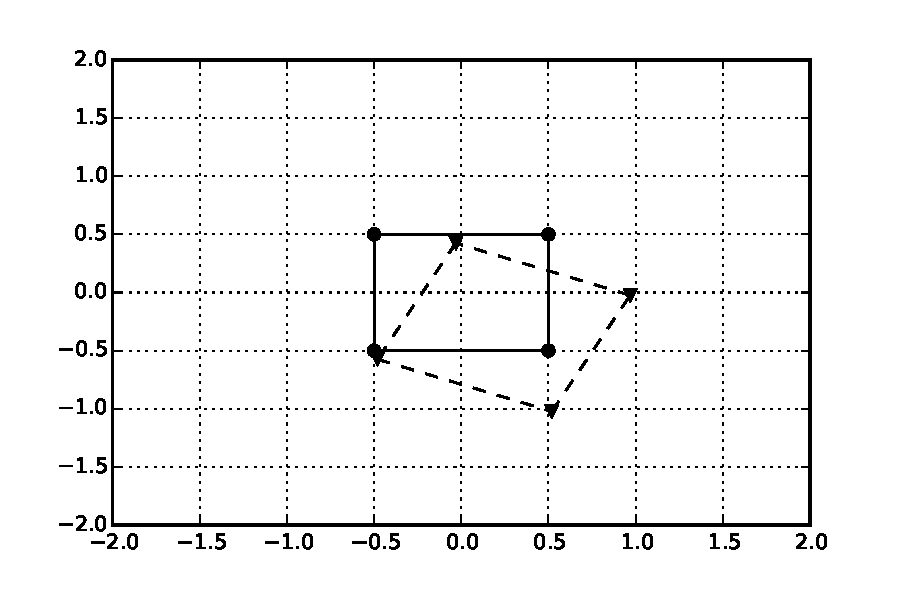
\includegraphics[width=\textwidth]{first.pdf}
		\caption{$\lambda_1 = 0$. }
	\end{subfigure}\,
%
	\begin{subfigure}[b]{0.450\textwidth}\qquad
		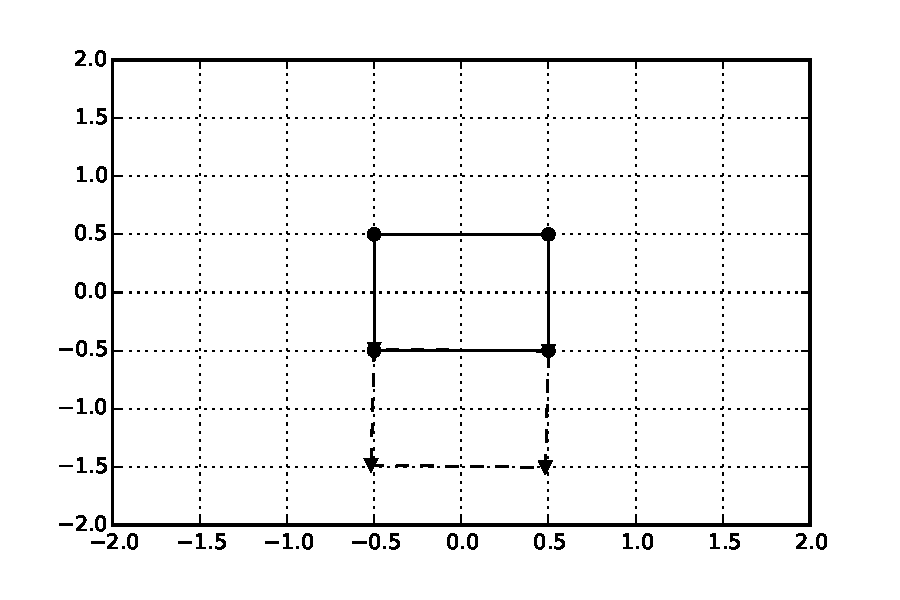
\includegraphics[width=\textwidth]{second.pdf}
		\caption{$\lambda_2 = 0$.}
	\end{subfigure}\\
%
\centering
	\begin{subfigure}[b]{0.450\textwidth}\qquad
		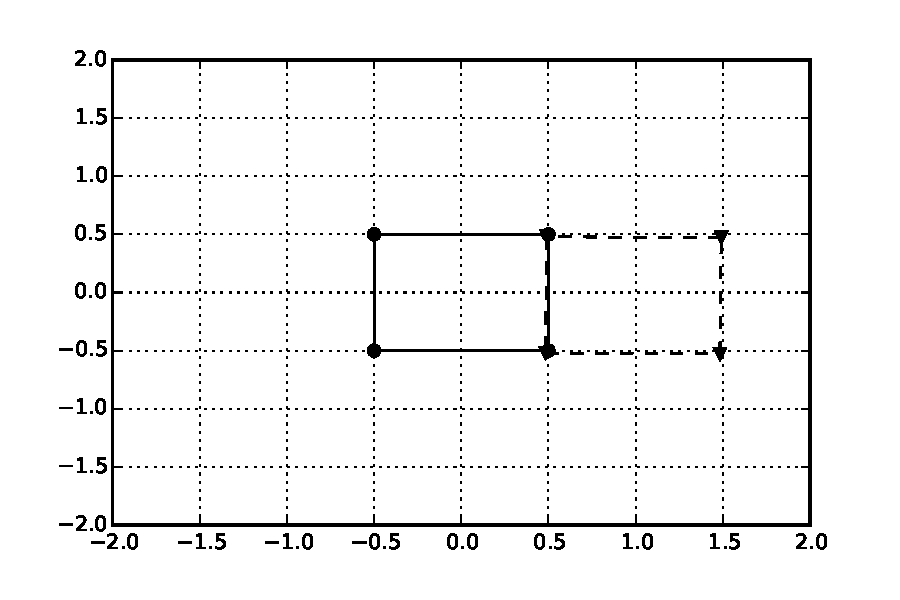
\includegraphics[width=\textwidth]{third.pdf}
		\caption{$\lambda_3 = 0$.}
	\end{subfigure}\,
%
	\begin{subfigure}[b]{0.450\textwidth}\qquad
		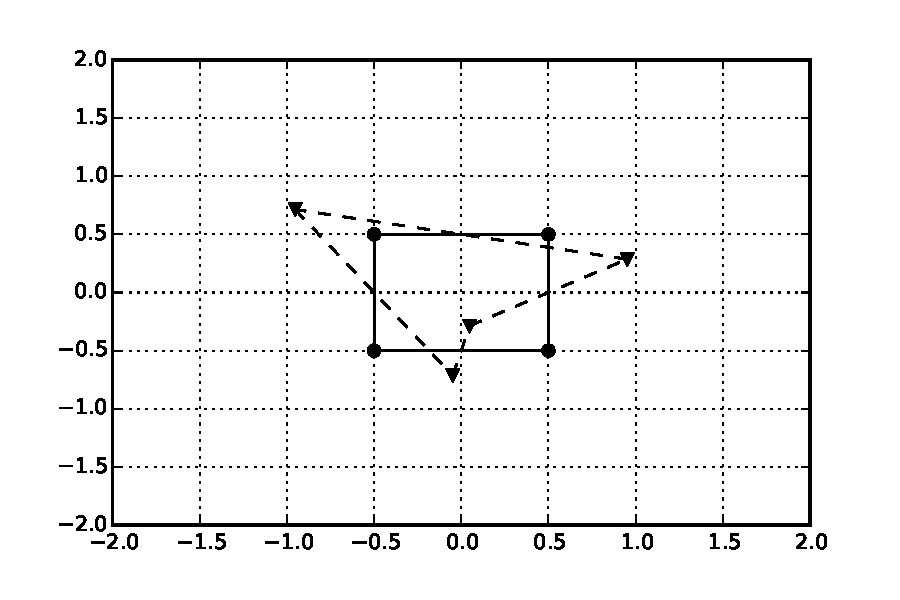
\includegraphics[width=\textwidth]{fourth.pdf}
		\caption{$\lambda_4 = 0.495$.}
	\end{subfigure}\\
%
\centering
	\begin{subfigure}[b]{0.450\textwidth}\qquad
		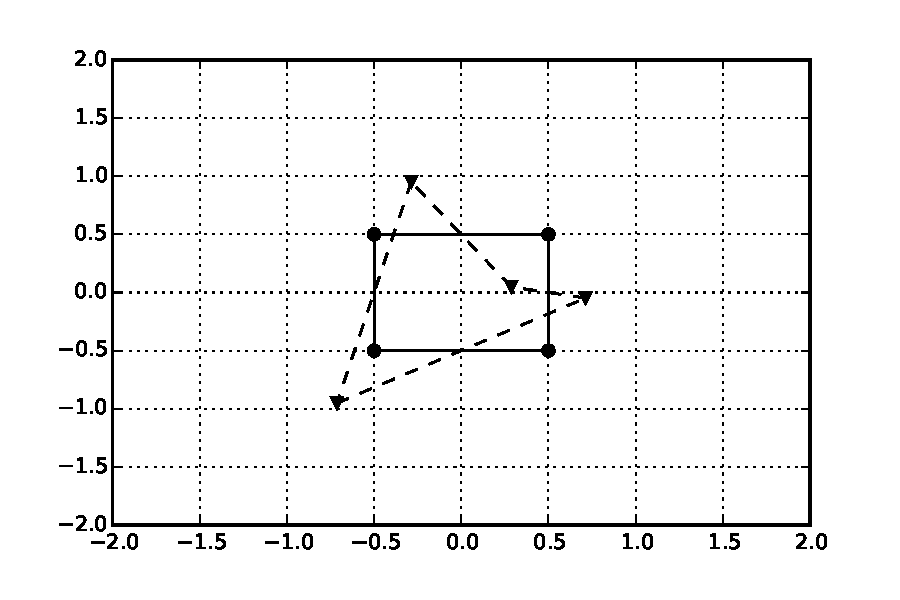
\includegraphics[width=\textwidth]{fifth.pdf}
		\caption{$\lambda_5 = 0.495$.}
	\end{subfigure}\,
%
	\begin{subfigure}[b]{0.450\textwidth}\qquad
		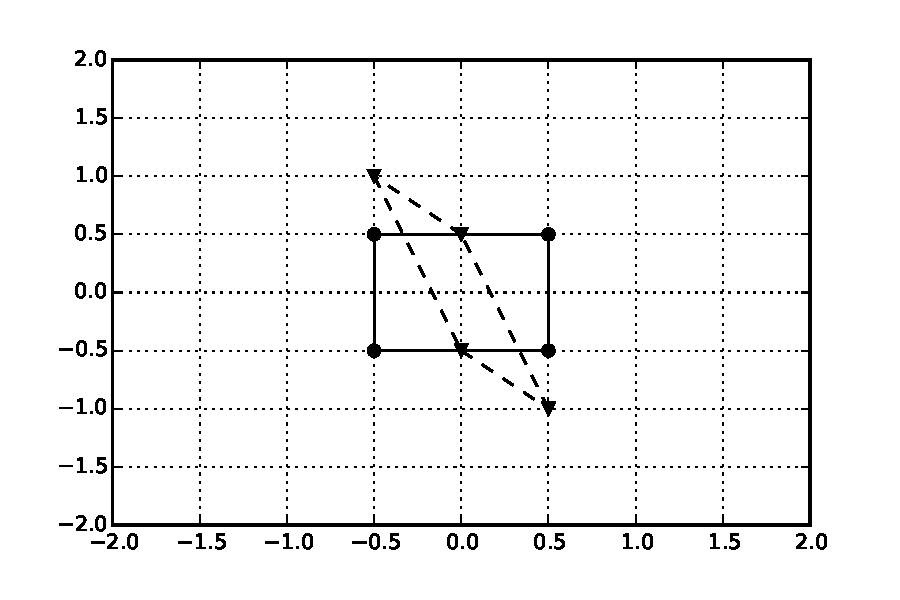
\includegraphics[width=\textwidth]{sixth.pdf}
		\caption{$\lambda_6 = 0.769$.}
	\end{subfigure}\\
%
\centering
	\begin{subfigure}[b]{0.450\textwidth}\qquad
		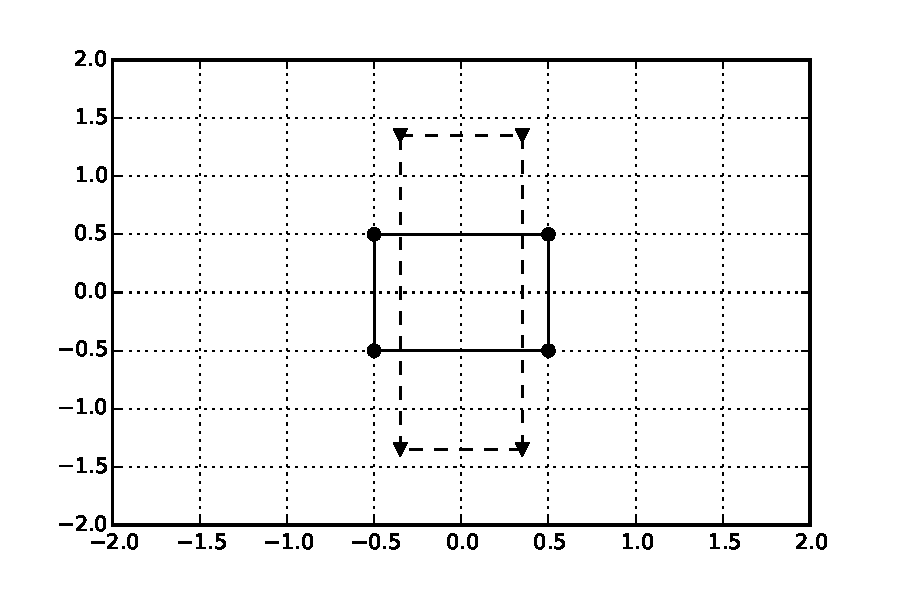
\includegraphics[width=\textwidth]{seventh.pdf}
		\caption{$\lambda_7 = 0.769$.}
	\end{subfigure}\,
%
	\begin{subfigure}[b]{0.450\textwidth}\qquad
		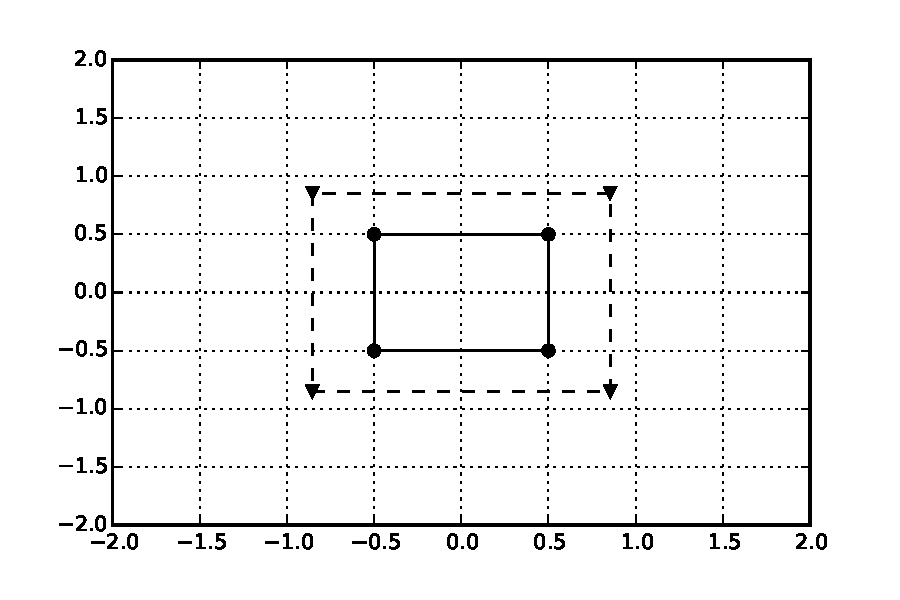
\includegraphics[width=\textwidth]{eight.pdf}
		\caption{$\lambda_8 = 1.43$.}
	\end{subfigure}
%
\caption{Deformation modes of a bi-linear element.}
\label{modos}
\end{figure}



\begin{figure}[H]
\centering
	\begin{subfigure}[b]{0.450\textwidth}\qquad
		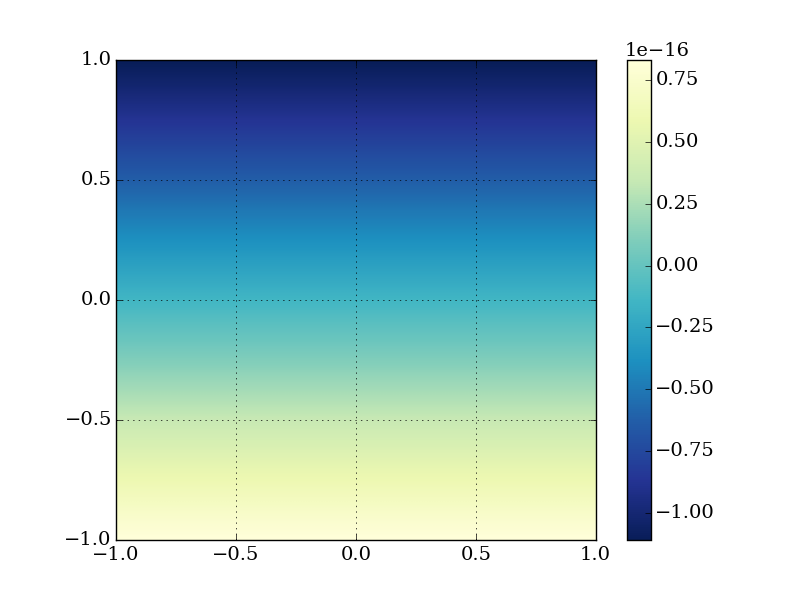
\includegraphics[width=\textwidth]{epsilonx.png}
		\caption{$\epsilon_{xx}$.}
	\end{subfigure}\,
%
	\begin{subfigure}[b]{0.450\textwidth}\qquad
		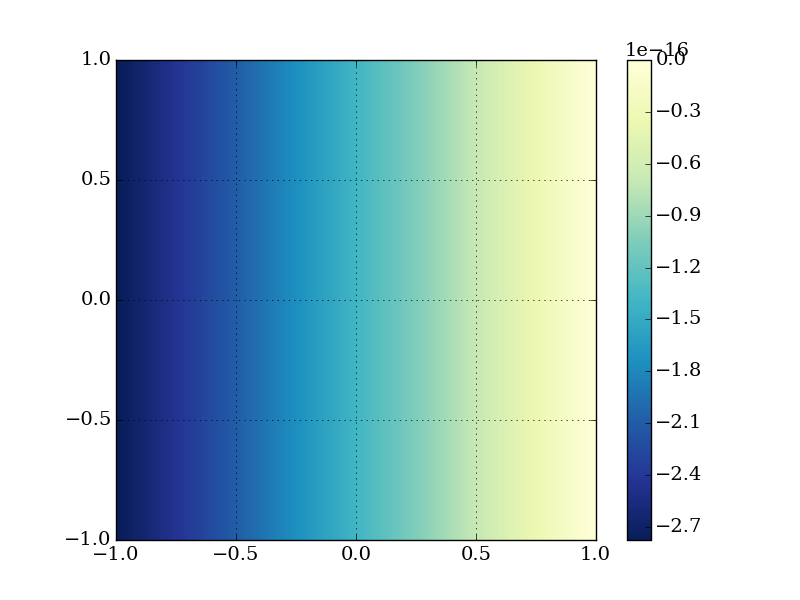
\includegraphics[width=\textwidth]{epsilony.png}
		\caption{$\epsilon_{yy}$.}
	\end{subfigure}
	\begin{subfigure}[b]{0.450\textwidth}\qquad
		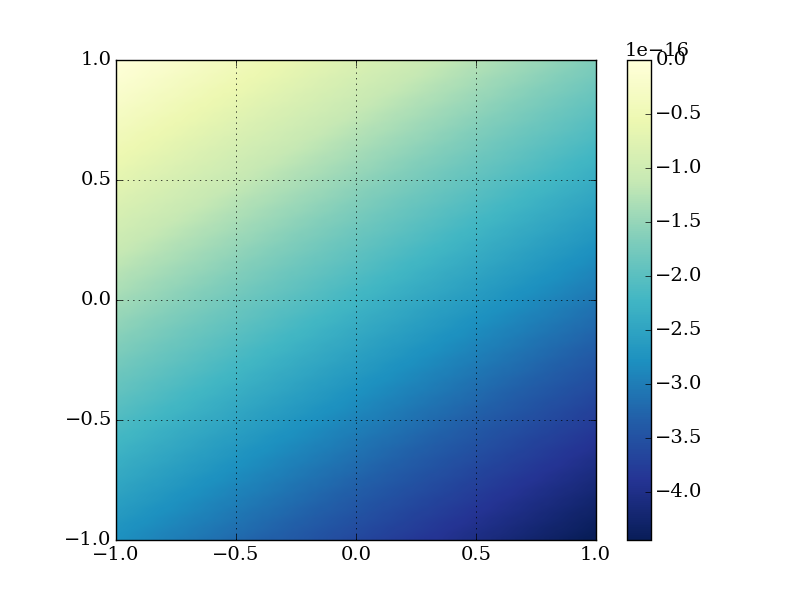
\includegraphics[width=\textwidth]{gammaxy.png}
		\caption{$\gamma_{xy}$}
	\end{subfigure}
%
\caption{Deformation modes of a bi-linear element.}
\label{strains}
\end{figure}



\section{Analysis of the mesh results}

Consider the square energy norm of the error $\left\| {{{\vec e}_h}} \right\|_E^2$. This error satisfies

\[\left\| {{{\vec e}_h}} \right\|_E^2 > 0\]

and will be used as an error estimate of the accuraccy of the finite element solution. Particularly we will use the following relationship (see \cite{abaqus1989karlsson})

\begin{equation}
\left\| {{{\vec e}_h}} \right\| \le \alpha {h^k}
\label{estimate1}
\end{equation}


from which we can write:


\begin{equation}
\log \left\| {{{\vec e}_h}} \right\| \approx \log \alpha  + k\log h
\label{estimate2}
\end{equation}

In \cref{estimate2} $k$ is the order of the complete interpolation polynomial present in the mesh and gives a measure of the order of convergence in the finite element solution, while the rate of convergency is given by $\alpha$.

In order to conduct the convergency study we perform a series of finite element analysis. For each mesh we compute $\left\| {\vec u - {{\vec u}_h}} \right\|$ which is equivalent to $\vec e_h$ and where $\vec u$ is the exact solution. In order to find the exact solution we assume that the most refined results have functionals corresponding to ${\Pi _{n - 2}}$, ${\Pi _{n - 1}}$ and ${\Pi _{n}}$ from which:

\[{\Pi _{Exa}} = \frac{{\Pi _{n - 1}^2 - {\Pi _n}{\Pi _{n - 2}}}}{{(2{\Pi _{n - 1}} - {\Pi _n} - {\Pi _{n - 2}})}}\]

The procedure is summarized below:

\begin{itemize}
\item Solve a series of meshes with solutions given by $\vec u_1, \vec u_2,...,\vec u_n$. Each mesh has a characteristic element size $h$.
\item For each mesh find the total potential energy:

\[{\Pi_h} =  - \frac{1}{2}{U^T}KU\]

\item Using the most refined meshes compute the potential energy for the exact solution:

\[{\Pi _{Exa}} = \frac{{\Pi _{n - 1}^2 - {\Pi _n}{\prod _{n - 2}}}}{{2{\Pi _{n - 1}} - {\Pi _n} - {\Pi _{n - 2}}}}\]

\item For each mesh compute:

\[\frac{{\left\| {{{\vec u}_{Exa}} - {{\vec u}_h}} \right\|}}{{\left\| {{{\vec u}_{Exa}}} \right\|}} = {\left[ {\frac{{{\Pi _{Exa}} - {\Pi _h}}}{{{\Pi _{Exa}}}}} \right]^{1/2}}\]

and fill out the following table:

\begin{center}
\begin{tabular}{ |c|c|c|c| }
  \hline
  $h$ & ${\prod _{FE}}$ & $\left\| {{{\vec u}_{Exa}} - {{\vec u}_{FE}}} \right\|$ & $\frac{{\left\| {{{\vec u}_{Exa}} - {{\vec u}_{FE}}} \right\|}}{{\left\| {{{\vec u}_{Exa}}} \right\|}}$ \\
  \hline 
  $1.0$  & $$ & $$  & $$  \\
  \hline
   $0.5$  & $$ & $$  & $$  \\
  \hline
   $0.25$  & $$ & $$  & $$  \\
  \hline
   $ 0.125$  & $$ & $$  & $$  \\
  \hline
  $ 0.0625$  & $$ & $$  & $$  \\
  \hline
\end{tabular}
\captionof{table}{Convergence of anlysis results}
\label{tabconv}
\end{center}


\item Plot the values of $\log \left( {\frac{{\left\| {{{\vec u}_{Exa}} - {{\vec u}_h}} \right\|}}{{\left\| {{{\vec u}_{Exa}}} \right\|}}} \right)$ vs $\log h$ and determine the slope which upon convergence must be close to the order of the complete polynomial used in the discretization.

\end{itemize}


\paragraph*{Exampla: bar in compression}
\Cref{mallas} shows a tappered bar under a compressive uniformly distributed load of total magnitude $P=0.5$. The bar is of length $l=10$ and its large and short ends given by $h_1 = 2.0$ and $h_2 =0.5$ respectively. The material properties correspond to a Poisson's ratio and Young modulos $\nu=0.30$ and $E=1.0$. We want to find the converged solution for the bar after using 3-noded triangular elements.



\begin{figure}[H]
\centering
	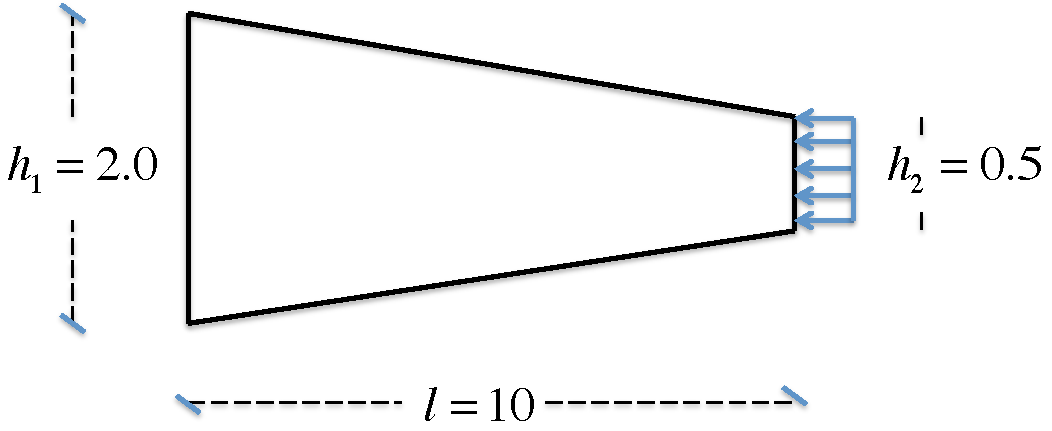
\includegraphics[width=5.0 in]{img/tappered.pdf}	
	\label{bar}
	\caption{Tappered bar under compressive load at the tip.}
\end{figure}

\Cref{mallas} displays 4 consecutive meshes with decreasing element size namely $h=[1.0, 0.5, 0.25, 0.125]$. While \cref{gamatap} displays the shear strain contour maps for the finite element solutions corresponding to the coarse and refined meshes. It is clear how these contours become smooth as the mesh is refined. This approach is sometimes used as an empirical test of convergence.

To measure the finite element convergence we first compute the total potential energy in each mesh ccording to:

\[{\Pi _{FE}} =  - \frac{1}{2}{U^T}KU.\]

Now assuming we have consecutive meshes each one obtained after halving the elements in the previous mesh we have the following approximation for the exact total potential energy of the system, computed the last most refined meshes:

\[{\Pi _{Exa}} = \frac{{{{1.161}^2} - ( - 1.160)( - 1.155)}}{{ - 2(1.161) - ( - 1.160) - ( - 1.155)}} = -1.160.\]

To compute the energy norm of the error we use:

\[\frac{{\left\| {{{\vec u}_{Exa}} - {{\vec u}_{FE}}} \right\|}}{{\left\| {{{\vec u}_{Exa}}} \right\|}} = {\left[ {\frac{{{\Pi _{Exa}} - {\prod _{FE}}}}{{{\Pi _{Exa}}}}} \right]^{1/2}}.\]

The analysis results are reported in \cref{ejemplo}.

%\begin{figure}[H]
%\centering
%	\subfloat [$h=1.00$]{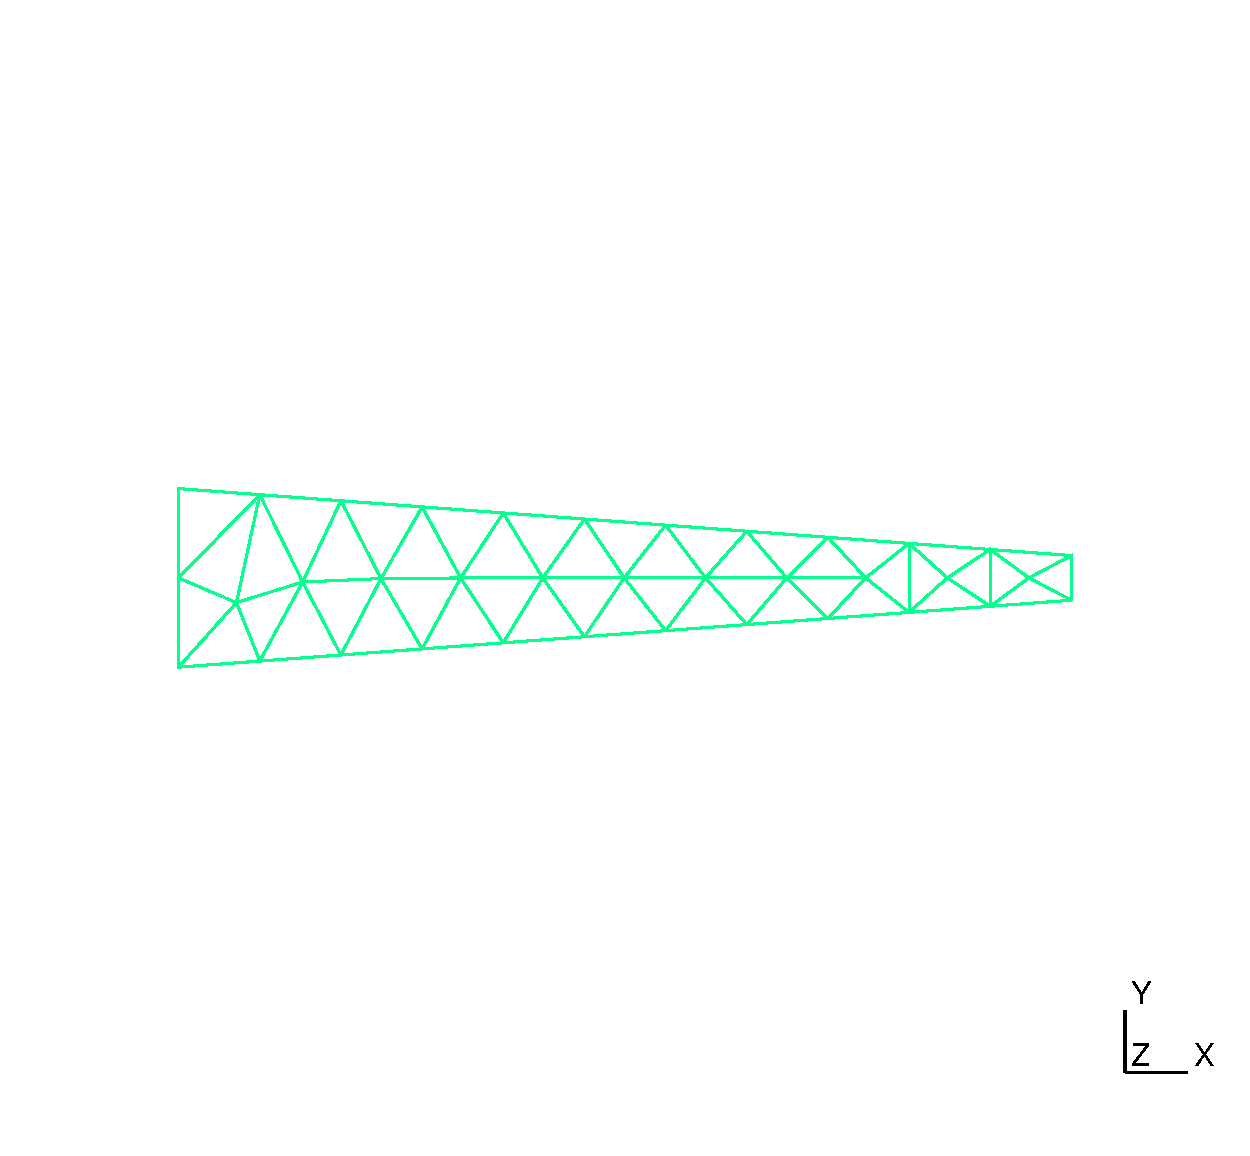
\includegraphics[width=2.5 in]{tap1.pdf}}
%	\subfloat [$h=0.50$]{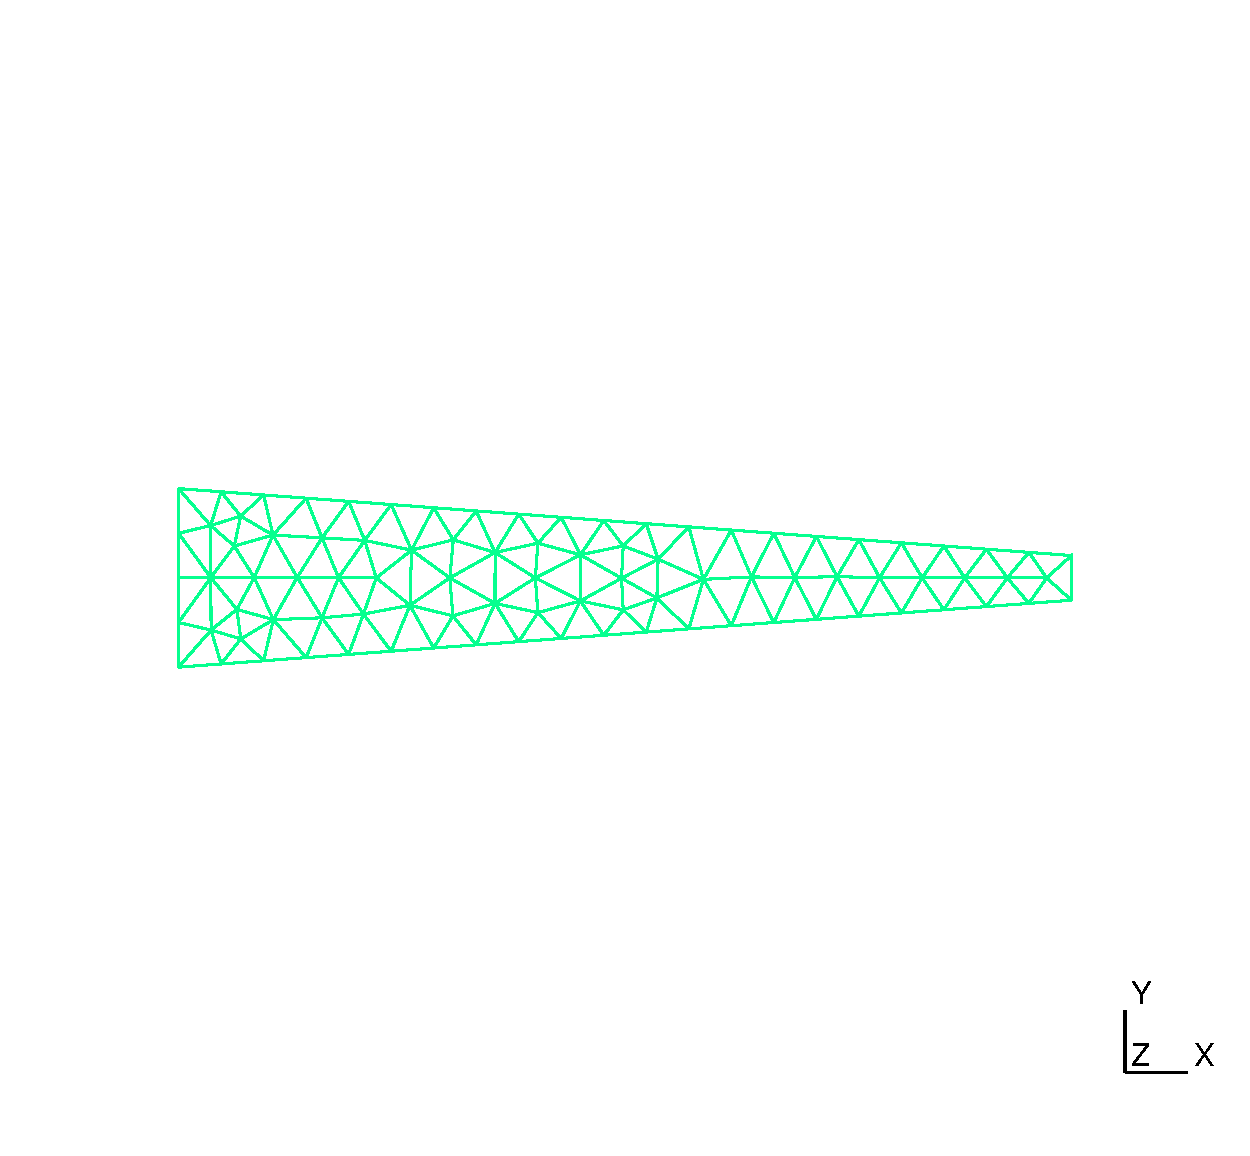
\includegraphics[width=2.5 in]{tap2.pdf}}\\
%%	\vspace{-.2 cm}
%	\subfloat [$h=0.250$]{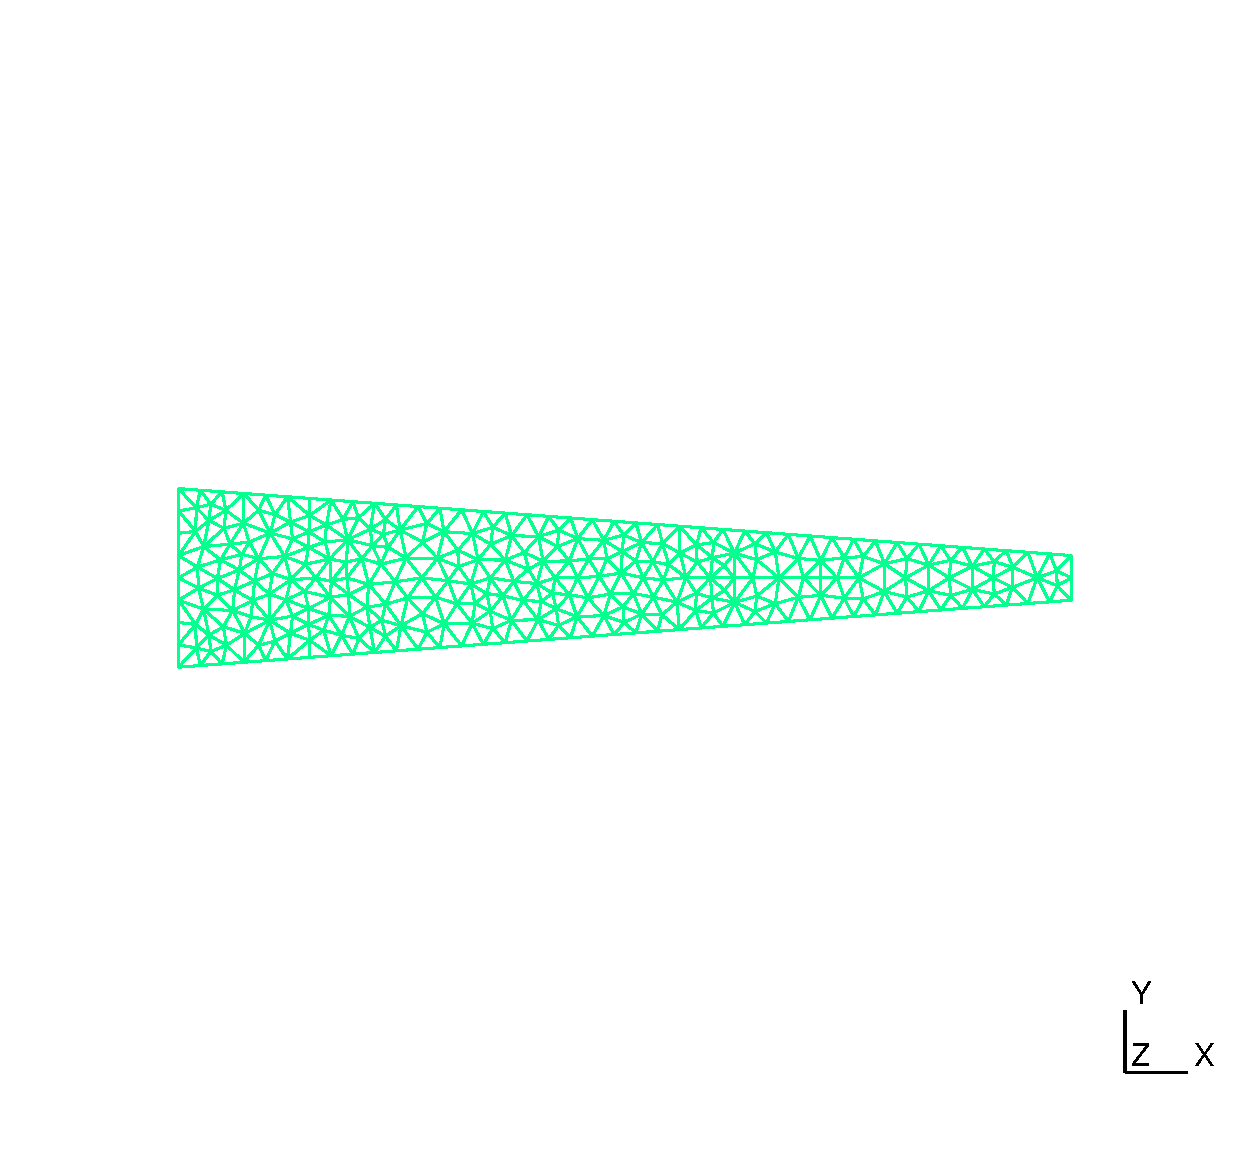
\includegraphics[width=2.5 in]{tap3.pdf}}
%	\subfloat [$h=0.125$]{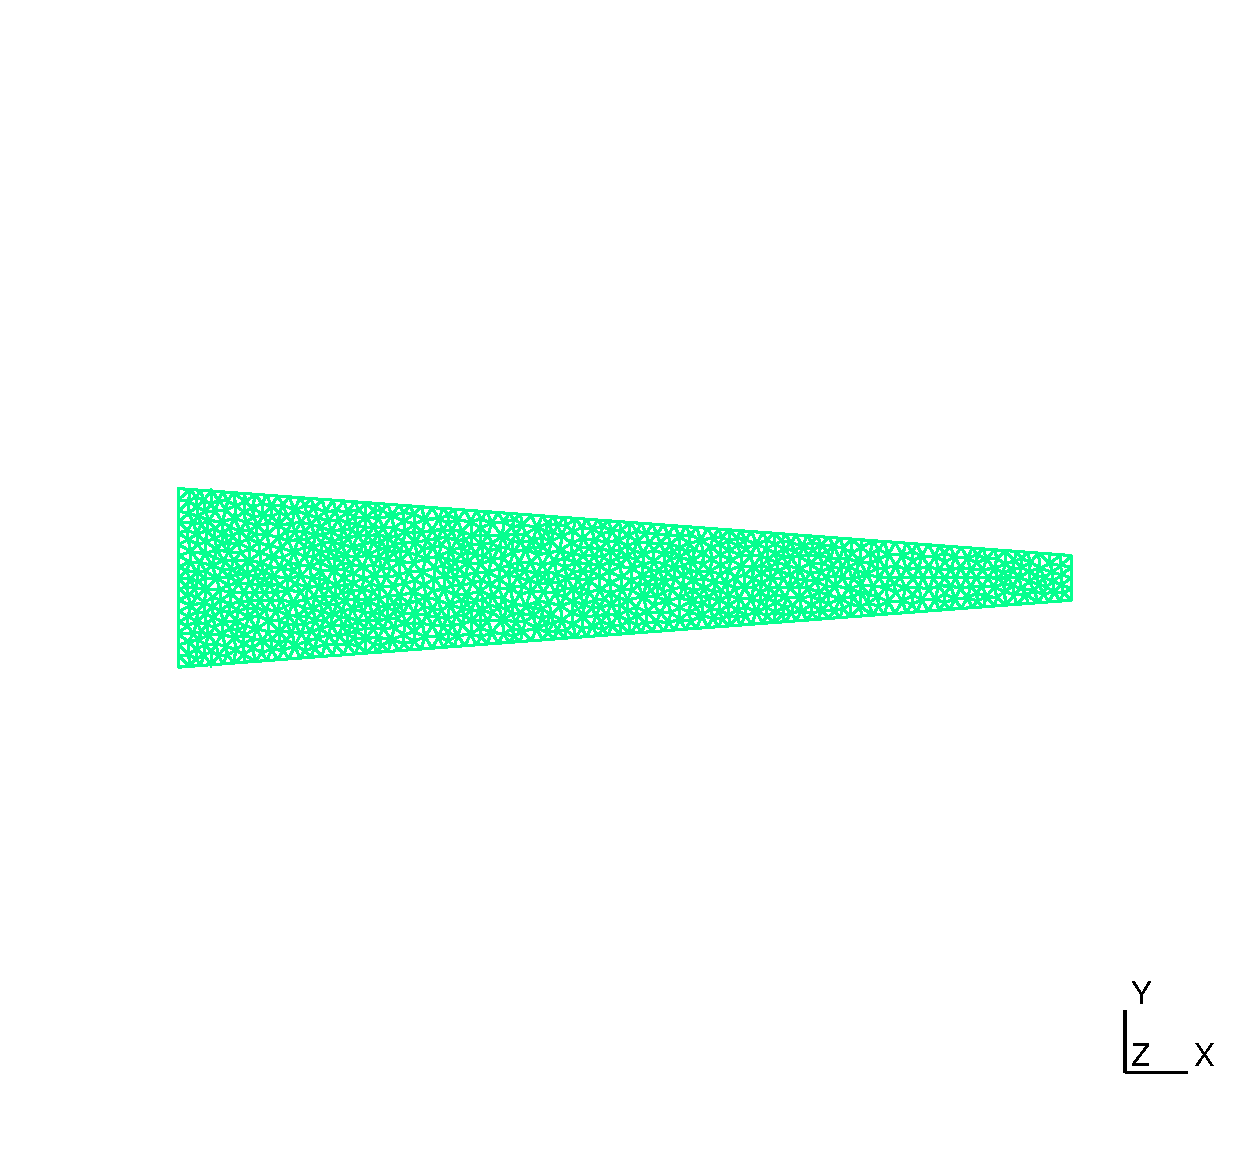
\includegraphics[width=2.5 in]{tap4.pdf}}\\
%	\caption{Refined meshes for a tappered bar.}
%	\label{mallas}
%\end{figure}


%%%%%
\begin{figure}[H]
\centering
	\begin{subfigure}[b]{0.450\textwidth}\qquad
		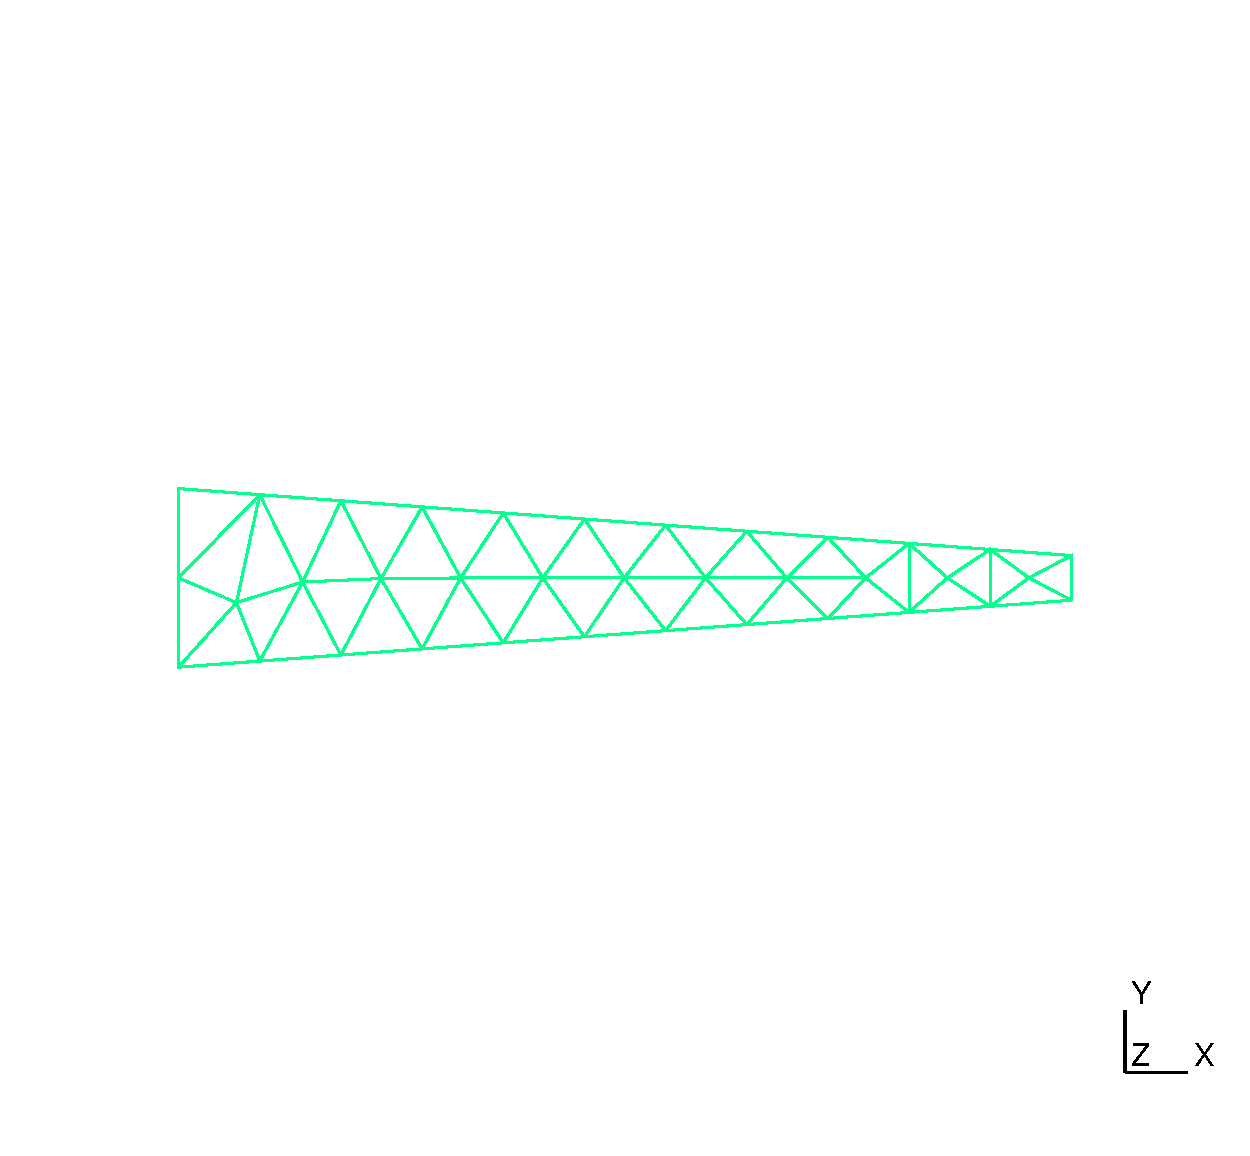
\includegraphics[width=\textwidth]{tap1.pdf}
		\caption{$h=1.00$. }
	\end{subfigure}\,
%
	\begin{subfigure}[b]{0.450\textwidth}\qquad
		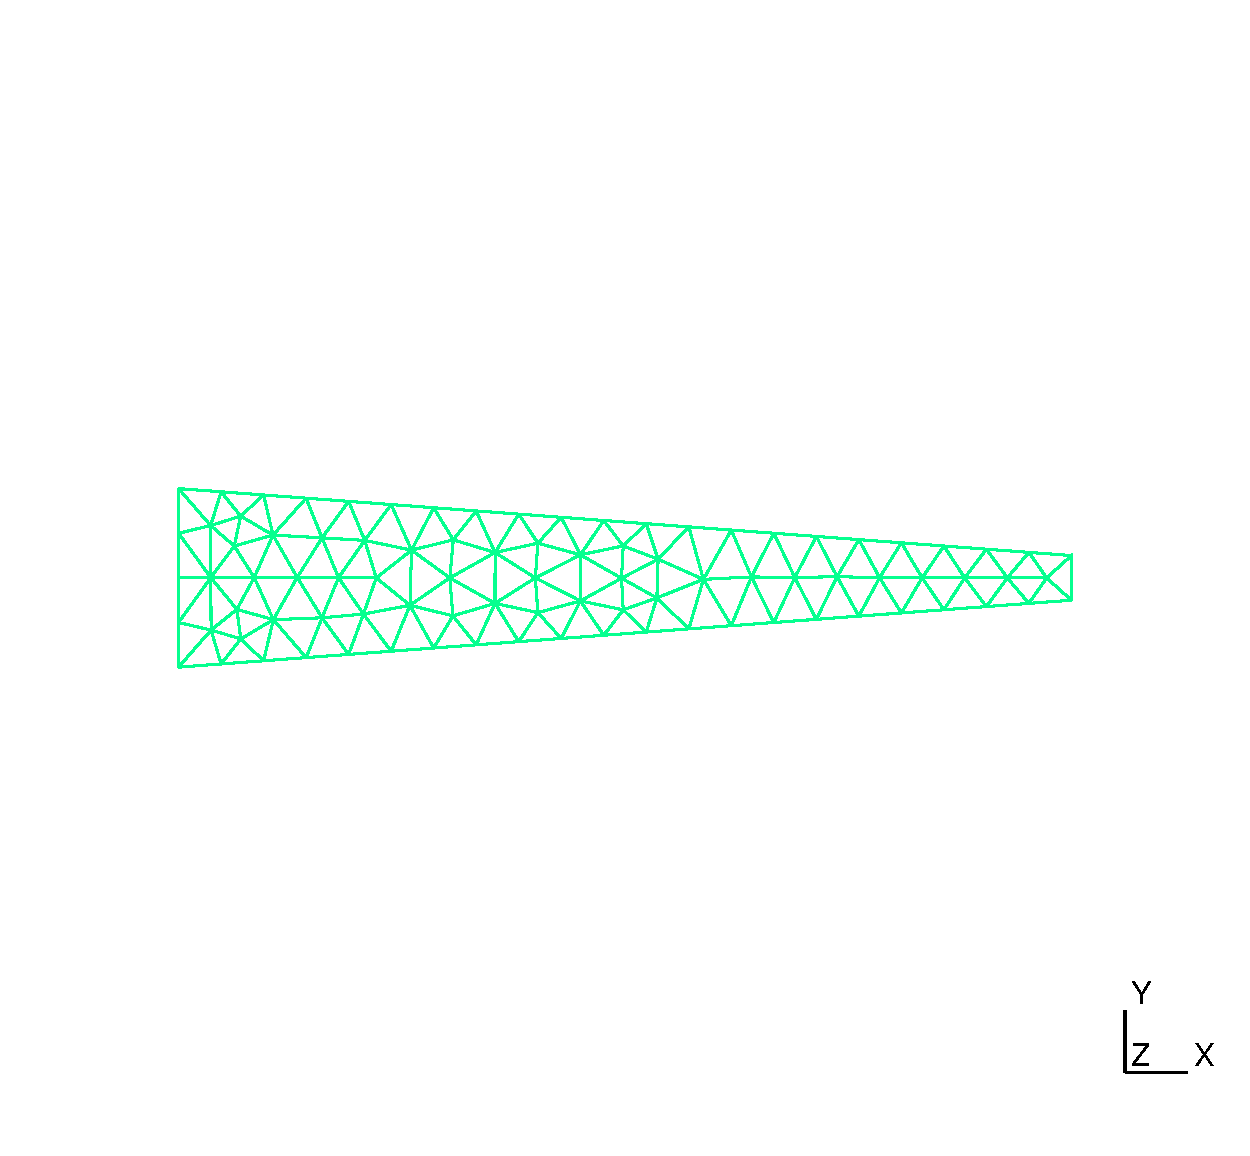
\includegraphics[width=\textwidth]{tap2.pdf}
		\caption{$h=0.50$.}
	\end{subfigure}\\
%
\centering
	\begin{subfigure}[b]{0.450\textwidth}\qquad
		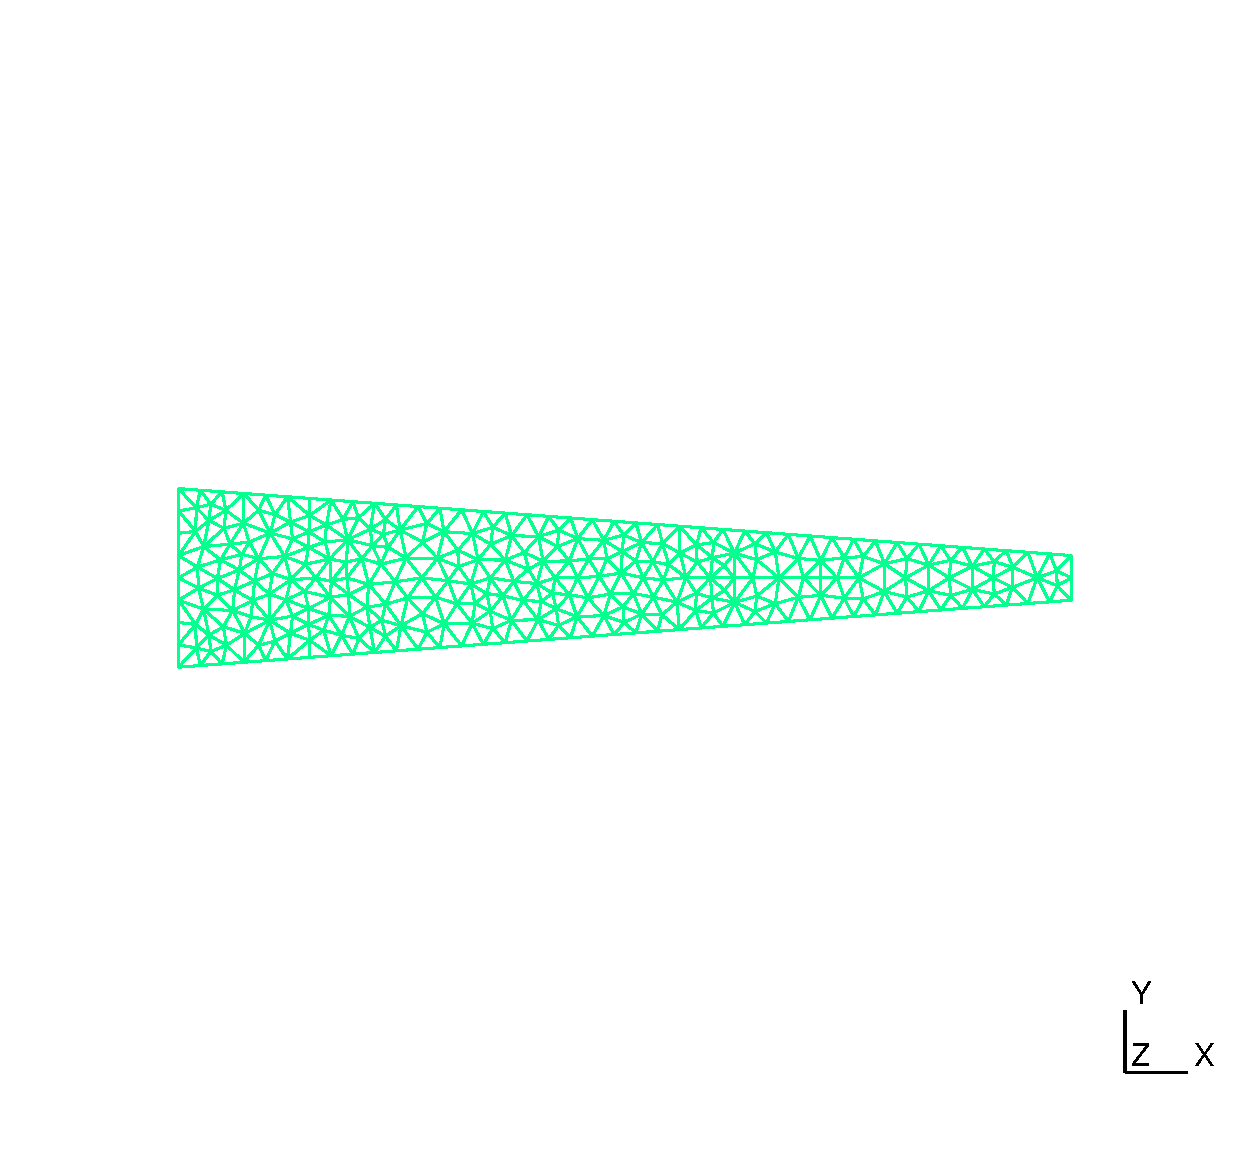
\includegraphics[width=\textwidth]{tap3.pdf}
		\caption{$h=0.250$.}
	\end{subfigure}\,
%
	\begin{subfigure}[b]{0.450\textwidth}\qquad
		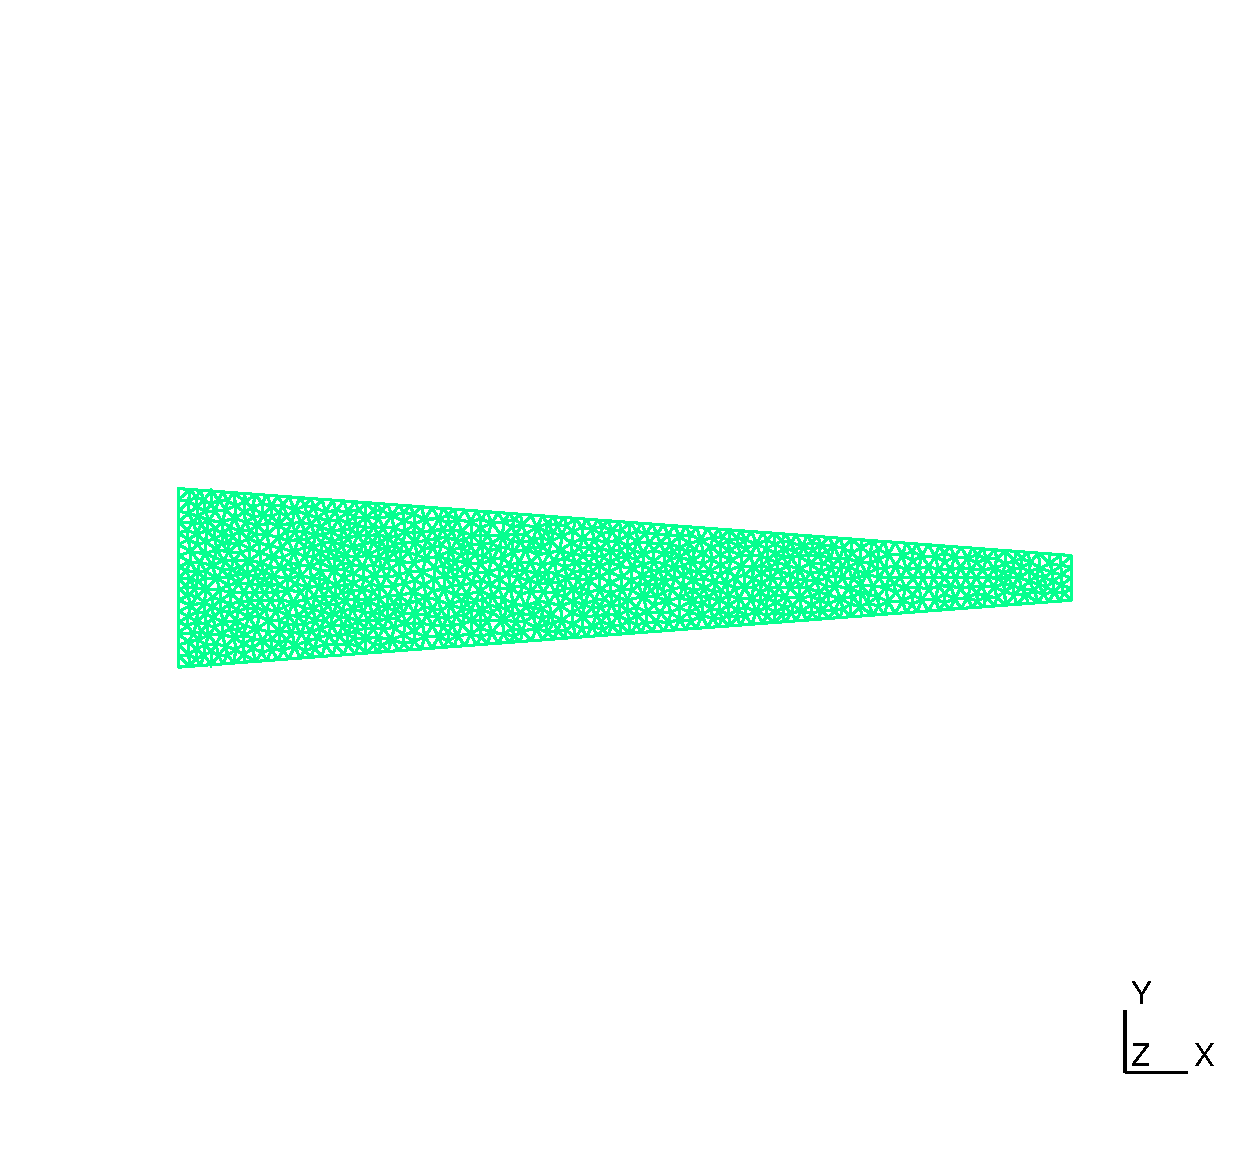
\includegraphics[width=\textwidth]{tap4.pdf}
		\caption{$h=0.125$.}
	\end{subfigure}
%
\caption{Refined meshes for a tappered bar.}
\label{mallas}
\end{figure}


\begin{figure}[H]
\centering
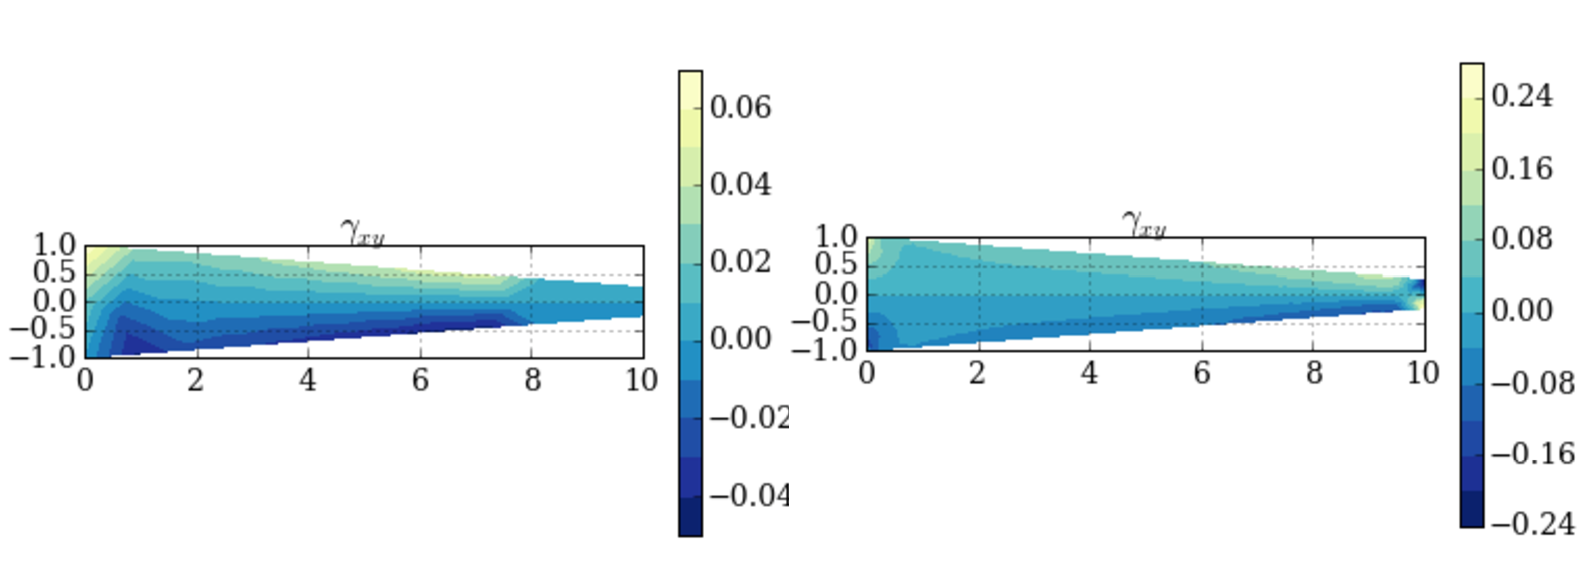
\includegraphics[width=6 in]{gamatap.pdf}
\caption{Shear strain distribution for the coarse and fine mesh.}
\label{gamatap}
\end{figure}


%%%%%%


\begin{center}
\begin{tabular}{cccc}
  \hline
  $h$ & ${\Pi _{FE}}$ & $\left\| {{{\vec u}_{Exa}} - {{\vec u}_{FE}}} \right\|$ & $\frac{{\left\| {{{\vec u}_{Exa}} - {{\vec u}_{FE}}} \right\|}}{{\left\| {{{\vec u}_{Exa}}} \right\|}}$ \\
  \hline 
  $1.0$      & $-1.151$ & $0.095$  & $0.088$  \\
   $0.5$     & $-1.155$ & $0.071$  & $0.066$  \\
   $0.25$    & $-1.161$ & $0.032$  & $0.030$  \\
   $ 0.125$  & $-1.160$ & $0.001$  & $0.001$  \\
  \hline
\end{tabular}
\captionof{table}{Convergence of anlysis results}
\label{ejemplo}
\end{center}

To measure convergence we plot:
\[\log \left( {\left\| {{{\vec u}_{Exa}} - {{\vec u}_{FE}}} \right\|} \right) = 
\log c + k\log h\]
leading to \cref{fig:conv} from which  $k \approx 1.14.$
\begin{figure}[H]
\centering
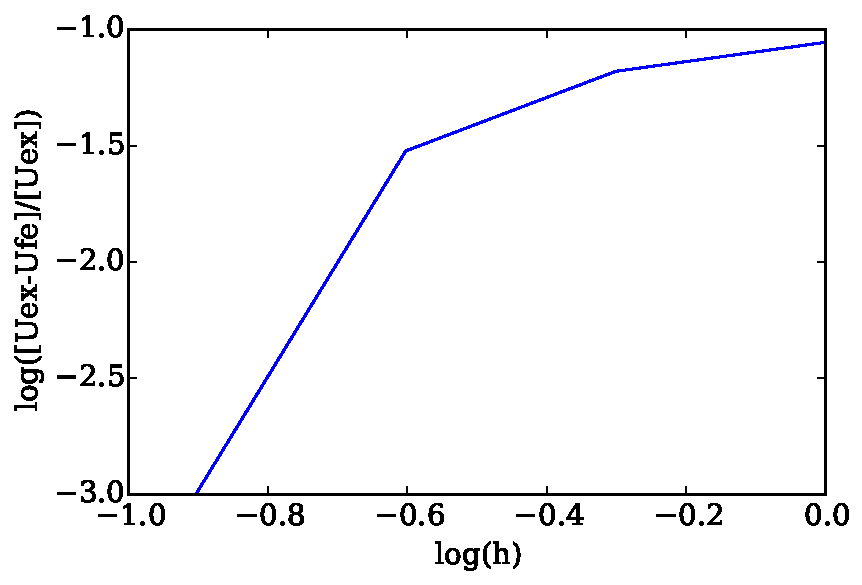
\includegraphics[width=0.65\textwidth]{img/conver.pdf}
\caption{Energy norm of the error}
\label{fig:conv}
\end{figure}

\newpage


\paragraph*{Example: cantilever beam}
Consider the cantilever beam shown in \cref{fig:viga}

\begin{figure}[H]
\centering
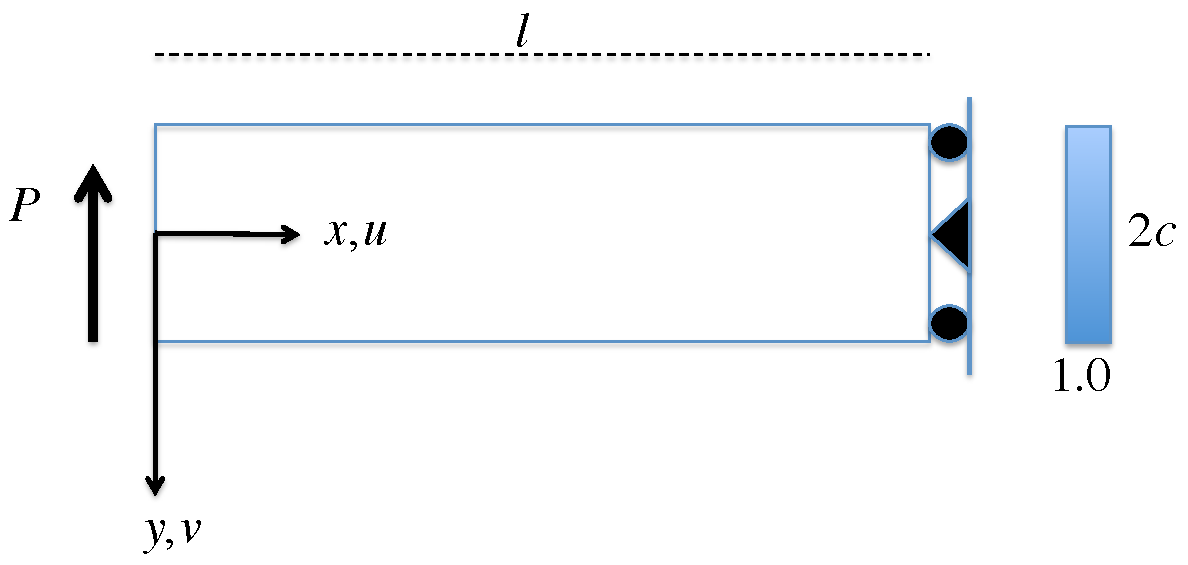
\includegraphics[width=0.75\textwidth]{img/beam.pdf}
\caption{Cantelever beam.}
\label{fig:viga}
\end{figure}
with analytic solution \citep{book:timoshenko} given by:
\begin{align*}
u &=  -\frac{P}{2EI} x^2 y - \frac{\nu P}{6EI} y^3 + \frac{P}{2IG}{y^3} + 
\left(\frac{P l^2}{2EI} - \frac{P c^2}{2IG}\right)y \, ,\\
v &= \frac{\nu P}{2EI} x y^2 + \frac{P}{6EI} x^3 - 
\frac{Pl^2}{2EI}x + \frac{Pl^3}{3EI}\, ,\\
\varepsilon_{xx} &= \pdv{u}{x} \equiv - \frac{P}{EI}xy\, ,\\
\varepsilon_{yy} &= \pdv{v}{y} \equiv \frac{\nu P}{EI} xy\, ,\\
\gamma_{xy} &= \pdv{u}{y} + \pdv{v}{x} \equiv \frac{P}{2IG} (y^2 - c^2)\, .
\end{align*}

The horizontal and vertical displacement field corresponding to the particular 
values of $E=1000.0$, $\nu=0.30$ for the material parameters; $l=24$ and $2c=8$ 
for the geometry and $P=50$ (upwards) for the load is shown below:
\begin{figure}[H]
\centering
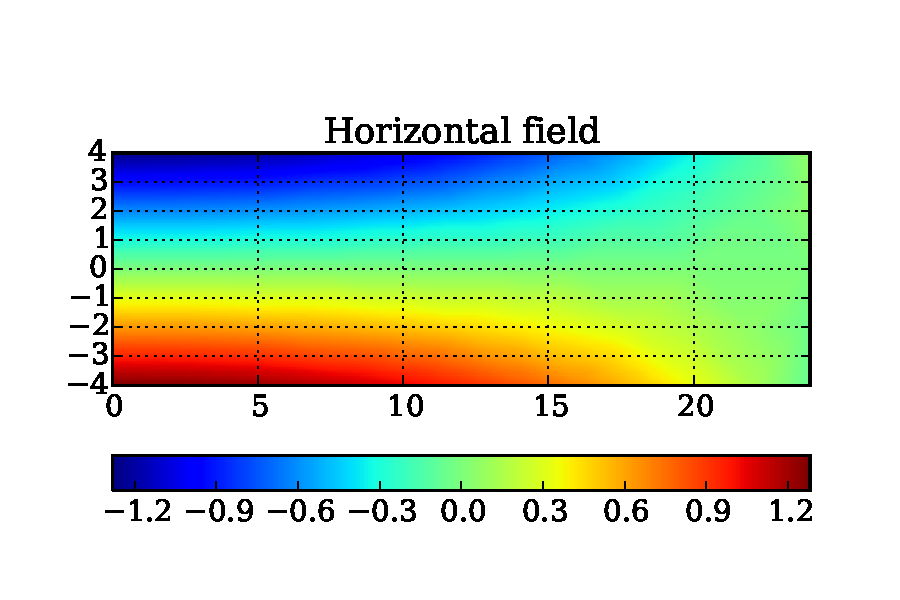
\includegraphics[width=0.75\textwidth]{img/anahorizo.pdf}\\
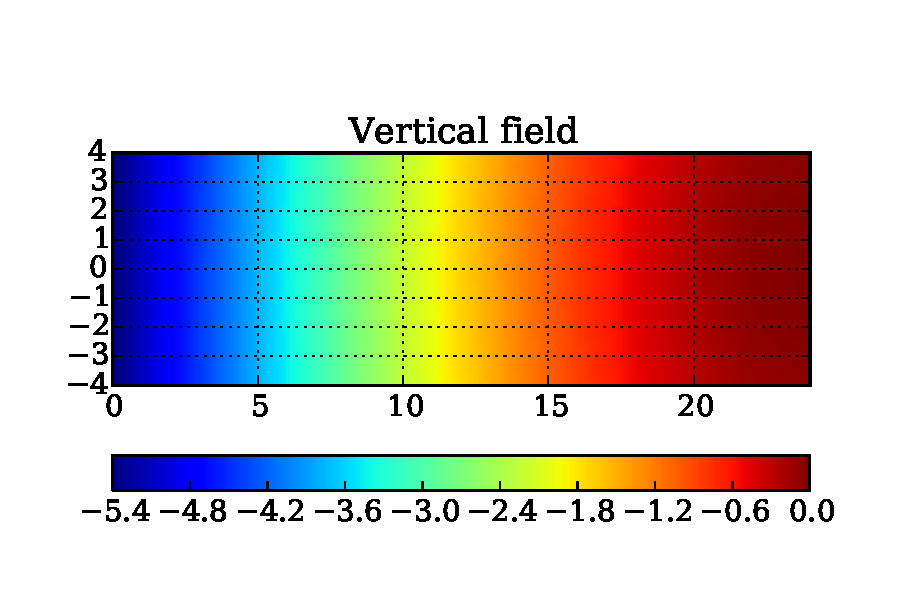
\includegraphics[width=0.75\textwidth]{img/anavertic.pdf}
\caption{Displacement field for the cantilever beam.}
\label{fig:ecuacion}
\end{figure}


Perform a finite element simulation using a series of refined meshes with charateristic element size corresponding to $h=[6.0,3.0,1.5,0.75,0.375]$ and show that convergence is achieved. To conduct the finite element analysis fill out \cref{problem}


\begin{center}
\begin{tabular}{cccc}
\hline
$h$ & $\prod_{FE}$ & $\left\| \vec{u}_{Exa} - \vec{u}_{FE}\right\|$ 
& $\frac{\left\| \vec{u}_{Exa} - \vec{u}_{FE}\right\|}{\left\| 
\vec{u}_{Exa} \right\|}$ \\
\hline 
$6.0$  & $$ & $$  & $$  \\
$3.0$  & $$ & $$  & $$  \\
$1.5$  & $$ & $$  & $$  \\
$ 0.75$  & $$ & $$  & $$  \\
$ 0.375$  & $$ & $$  & $$  \\
\hline
\end{tabular}
\captionof{table}{Convergence of anlysis results}
\label{problem}
\end{center}